 \documentclass[12pt]{report}
\usepackage[utf8]{inputenc}
\usepackage[T1]{fontenc}
\usepackage[a4paper,left=2cm,right=2cm,top=2cm,bottom=2cm]{geometry}
\usepackage[frenchb]{babel}
\usepackage{libertine}
\usepackage{amsmath,amssymb,hyperref,array,xcolor,multicol,verbatim,mathpazo,url}
\usepackage[normalem]{ulem}
\usepackage[pdftex]{graphicx}
\usepackage{float}
\usepackage{enumitem}
\usepackage{fancyhdr}
\usepackage{fullpage}
\usepackage{listings}
\usepackage{moreverb}
\usepackage{wrapfig}
\usepackage{setspace}
\usepackage{tikz}
\usepackage{subfigure}

\usetikzlibrary{arrows,shapes,positioning,shadows,trees}
\tikzstyle{abstract}=[rectangle, draw=black, rounded corners, fill=blue!40, drop shadow,
        text centered, anchor=north, text=white, text width=2.5cm]
\tikzstyle{comment}=[rectangle, draw=black, rounded corners, fill=green, drop shadow,
        text centered, anchor=north, text=white, text width=1.5cm]
\tikzstyle{myarrow}=[->, >=open triangle 90, thick]
\tikzstyle{line}=[-, thick]


\lstset{
numbers=left,
basicstyle=\normalsize,
upquote=true,
aboveskip={1.5\baselineskip},
columns=fullflexible,
showstringspaces=false,
extendedchars=true,
breaklines=true,
showtabs=false,
showspaces=false,
showstringspaces=false,
identifierstyle=\ttfamily,
keywordstyle=\color[rgb]{0,0,1},
commentstyle=\color[rgb]{0.133,0.545,0.133},
stringstyle=\color[rgb]{0.627,0.126,0.941},
}

\title{Projet Thermostat Intelligent}
\date{\today}                                           

\makeatletter
\let\thetitle\@title
\let\thedate\@date
\makeatother

\pagestyle{fancy}
\fancyhf{}
\cfoot{\thepage}
\renewcommand{\headrulewidth}{0pt}

\begin{document}

\begin{titlepage}
    \centering
    
    \begin{minipage}{0.48\textwidth} \begin{flushleft}
	
\includegraphics[scale = 0.6]{Logo.PNG}
	\end{flushleft}\end{minipage}
	\begin{minipage}{0.48\textwidth} \begin{flushright}
	
\includegraphics[scale = 0.6]{ULB.PNG}
	\end{flushright}\end{minipage}
    
    \vspace{6 cm}
    
    \textsc{\LARGE Universit\'{e} Libre de Bruxelles}\\[2.0 cm]
    \textsc{\Large TRANH-201 Projet Multidisciplinaire BA2}\\[0.5 cm]               
    \textsc{\large Groupe 22}\\[0.5 cm]               
    \rule{\linewidth}{0.2 mm} \\[0.4 cm]
    { \huge \bfseries \thetitle}\\
    \rule{\linewidth}{0.2 mm} \\[1.5 cm]
    
    \begin{minipage}{0.4\textwidth}
        \begin{flushleft} \large
            \emph{Auteurs:}\\
            \small DENGUIR Anass\\
			\small LOUHAJI Najlae\\
			\small NOEL Luca\\ 
			\small PHAN Trong Quy\\
            \end{flushleft}
            \end{minipage}~
            \begin{minipage}{0.4\textwidth}
            \begin{flushright} \large
            \emph{Superviseur:}\\
            \small VERMEIR Aur\'{e}lien\\
            \vspace{1 cm}
            \emph{Lecteur:}\\                                         
            \small VANSUMMEREN Stijn\\
        \end{flushright}
    \end{minipage}\\[2 cm]
    
    \vspace{1.5 cm}
    {\large \thedate}\\[2 cm]
 
    \vfill
    
\end{titlepage}

\tableofcontents

%%%%%%
%Attention les noms des chapitres et des sections ne sont pas définitifs, ajoutez-en ou modifier les si vous le jugez utile
%%%%%%
\newpage
\begin{center}
\large Abstract
\end{center}
\small \textbf{"Thermostat intelligent."} : par DENGUIR Anass, LOUHAJI Najlae, NOEL Luca, PHAN Trong Quy, TCHAMKAM NZINGA Marcel.\\
\newline
Cette ann\'{e}e, le projet orient\'{e} en informatique consiste en la conception d’un thermostat intelligent dont la principale fonction est d'assurer la régulation automatique de la température de plusieurs pièces par l’intermédiaire d’un thermostat central. Les tâches à réaliser consistent en la création d'un thermostat individuel fonctionnant sur base d'un circuit imprimé dénommé Arduino, la réalisation d'un serveur à partir d’un Raspberry Pi transmettant des instructions au thermostat individuel, l'élaboration  d’un protocole de communication entre les deux composantes (Arduino et Raspberry Pi), la modélisation de la régulation de la température d'un environnement et l’implémentation d’algorithmes rendant le thermostat autonome. L'Arduino et le Raspberry Pi sont fournis par l’Université. La régulation de la température est utilisée pour éviter des oscillations significatives de la température autour d’une consigne afin d'éviter une perte importante en énergie. Il en résultera pour chacune de ces tâches accomplies un thermostat (unité centrale) permettant l'installation de plusieurs thermostats individuels (asservis au thermostat principal).\\

Mots-clés:thermostat, Arduino, Raspberry Pi, régulation, serveur, communication.
\vspace{1.0cm}


\begin{center}
\large Abstract
\end{center}
\small \textbf{"Smart thermostat."} : by DENGUIR Anass, LOUHAJI Najlae, NOEL Luca, PHAN Trong Quy, TCHAMKAM NZINGA Marcel.\\
\newline
This year, the aim of the computer oriented project consists of disigning a smart thermostat which main function is the temperature automatic regulation of several room via a central thermostat.The different tasks ensure the creation of a thin thermostat with a Arduino, the production of a server on a Raspberry Pi sending each instruction to the thin thermostat, the preparation of  communication protocol between the two components (Arduino and Raspberry Pi), the temperature regulation modelling and the implementation of algorithms making the thermostat independant. The group responsible of this project was supplied by the university with the Arduino and the Raspberry Pi. The temperature regulation is used to avoid important variation of temperature when the environnement reaches a set temperature. The result of these accomplished tasks is a central thermostat that deals with an undefined number of thin thermostat.\\

Keywords: thermostat,Arduino,Raspberry Pi, regulation, server, communication



\chapter{Introduction}

Durant cette ann\'{e}e 2015-2016, le projet multidisciplinaire consiste en la conception d’un thermostat multi-zone et intelligent. Ce thermostat est l’association de plusieurs thermostats individuels, plac\'{e}s en des lieux attribu\'{e}s par l'utilisateur, envoyant leurs donn\'{e}es enregistr\'{e}es \`{a} un thermostat central. Celui-ci transmettra ses instructions aux thermostats individuels.

\noindent
Avant le commencement de la conception, un rapport de recherche bibliographique a dû être rendu. Ce rapport a permis au groupe de se baser sur plusieurs ouvrages et de juger la validit\'{e} des sources. Ce rapport a apporté les bases nécessaires à la compréhension du projet.\\

\noindent
Ce projet est décompos\'{e} en plusieurs \'{e}tapes :
\begin{itemize}
\item La r\'{e}alisation du thermostat individuel.
\item La conception d’un thermostat central avec algorithme de contr\^{o}le r\'{e}actif.
\item L’int\'{e}gration et validation du thermostat intelligent.
\item L'implémentation d’un algorithme de contr\^{o}le smart, c’est-\`{a}-dire optimiser le comportement du thermostat.
\end{itemize}
\vspace{0.45 cm}
\noindent
Il a \'{e}t\'{e} d\'{e}cid\'{e} de diviser ce rapport de mi-parcours en plusieurs parties d\'{e}crivant le d\'{e}roulement du projet :
\begin{itemize}
\item la conception, câblage et les aspects techniques du thermostat individuel
\item la gestion de la communication entre l’Arduino et le Raspberry Pi
\item la r\'{e}gulation de la temp\'{e}rature
\item la partie intelligente
\item le fonctionnement de groupe, compos\'{e} de la description de l’organisation du groupe
\end{itemize}
\vspace{0.45 cm}
Cette division en plusieurs chapitres permet une vision globale du projet ainsi qu'une lecture plus agr\'{e}able pour le lecteur. Ainsi, nous vous souhaitons une bonne lecture.

\begin{comment}
\chapter{Cahier des charges}
Dans le cadre de ce projet, il nous a été demandé de concevoir deux prototypes et ce chapitre aura pour but d'expliquer en premier lieu les différentes tâches et contraintes imposées dans le développement de ce projet. En effet, certains de ces objectifs permettent de mettre en avant les qualités de nos prototypes face aux thermostats traditionnels et le cahier des charges regroupent ces exigences.\\


\noindent
Le thermostat individuel doit être en mesure de:
\begin{enumerate}
\item \textbf{Détecter} une présence humaine,
\item \textbf{Mesurer} la température d'une pièce,
\item Lire l'\textbf{état} d'une vanne thermostatique,
\item \textbf{Actionner} l'ouverture et la fermeture d'une vanne thermostatique,
\item Transmettre \textbf{sans-fil} à l'unité centrale les informations liées à ses capteurs.
\end{enumerate}

\vspace{0.4 cm}

\noindent
Le thermostat central doit être capable de:
\begin{enumerate}
\item \^{E}tre \textbf{autonome},
\item Gérer un nombre \textbf{indéfini} de thermostats individuels afin d'assurer un système de \textbf{multi-zone}, 
\item \^{E}tre muni d'un \textbf{algorithme de contrôle} pour commander les vannes des thermostats satellites ainsi que recevoir les données de leurs capteurs,
\item Pouvoir \textbf{réguler la température de manière optimale} en fonction des caractéristiques de la pièce à chauffer,
\item Disposer d'un \textbf{tableau de bord} consultable depuis un navigateur web,
\end{enumerate}
\end{comment}

\chapter{Conception et aspect technique}
Dans ce chapitre, nous allons décrire brièvement les aspects physiques du prototype ainsi que les différents capteurs utilisés.

\section{Thermostat central}
Le thermostat central est constitué d'un Raspberry Pi 2 qui est un micro-ordinateur de faible coût. L'avantage de son utilisation est son faible prix et sa faible consommation électrique. Il est doté d'un dongle WiFi afin de générer un réseau WiFi et permettre une communication sans fil avec les différents thermostats satellites. C'est sur ce dernier qu'est implémenté l'algorithme de contrôle de la température et de gestion des thermostats individuels.

\section{Thermostat individuel}
Le thermostat individuel est constitué d'un Arduino Nano et est lié au thermostat central avec lequel il communique constamment via un protocole HTTP grâce à un module WiFI ESP8266 pré-configuré pour la transmission de requêtes.
Il est doté de deux capteurs, un thermistor et un capteur infrarouge, qui permettent respectivement de relever la température et la présence de personne dans une pièce.
Concernant leur fonctionnement, le capteur infrarouge envoie un signal électrique chaque fois qu'il détecte un mouvement tandis que le thermistor est une résistance qui varie en fonction de la température. \\

\begin{figure}[H]
    \begin{minipage}[t]{8cm}
    	\centering
        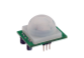
\includegraphics[scale=1.4]{detecteur_presence.png}
        \caption{\label{detecteur_presence.png} Détecteur de pr\'{e}sence}
    \end{minipage}\hfill
    \begin{minipage}[t]{8cm}
    	\centering
        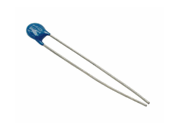
\includegraphics{thermistance.png}
        \caption{\label{thermistance} Thermistance}
    \end{minipage}
\end{figure}
\vspace{1cm}

Afin de récolter la température à partir du thermistor, nous avons recouru à une résistance de référence de 10k$\Omega$ et mis en place un pont diviseur de tension pour calculer la résistance du thermistor \cite{_types_????} et ainsi trouver la température grâce à la relation d’interpolation de Steinhart-Hart ci-dessous (\ref{Steinhart}). Dans la relation ci-dessous, A, B, C, D sont des constantes qui sont relatives au modèle de thermistance employé. Ces valeurs sont pr\'{e}sent\'{e}es dans le tableau des paramètres fournis par la compagnie Vishay\cite{100.pdf_????}\\

\vspace{0.5cm}
%\begin{equation}
%R(T) =R_{ref}^{A+\frac{B}{T}+\frac{C}{T^2}+\frac{D}{T^3}}
%\end{equation}
\textbf{Relation de Steinhart-Hart:}
\begin{equation}
\frac{1}{T(R)}=A+B\cdot\ln(\frac{R}{R_{ref}})+C\cdot\ln(\frac{R}{R_{ref}})^2+D\cdot\ln(\frac{R}{R_{ref}})^3
\label{Steinhart}
\end{equation}

\vspace{0.5cm}
La thermistance est plac\'{e}e en série avec la r\'{e}sistance de 10k$\Omega$ dans le circuit. On calculera donc la r\'{e}sistance de la thermistance à partir de la mesure de tension aux bornes de la résistance de référence par analyse d’un diviseur de tension. 
Afin de convertir les données reçues en bits par l'Arduino (entre 0 et 1023) en une tension, il suffit de la diviser par la valeur maximale en bits, 1023, et de multiplier le tout par la tension du générateur, en l'occurrence 5 volt. Nous pouvons ensuite calculer la résistance de la thermistance et obtenir la température avec la relation de Steinhart-Hart.\\
\vspace{0.5cm}

\textbf{Diviseur de tension (issu du syllabus de laboratoire de M. Haelterman \cite{haelterman_marc_physique_2014}):}

\begin{figure}[H]
\centering
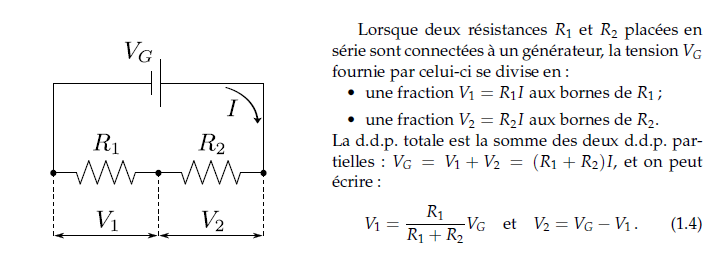
\includegraphics[scale=0.8]{divt.PNG}
\end{figure}

\section{Environnement de simulation}
L'environnement de simulation a été fourni par les organisateurs du projet. Celui-ci est constitué d'une résistance chauffante qui fait office de radiateur. L'actionnement de la valve est alors contrôlé via la transmission d'un courant modulé en amplitude (PWM) \cite{PWM} par le thermostat individuel. Il comporte également une entrée pour le branchement du capteur de température extérieur et permet d'alimenter le thermostat individuel. \\

\section{Plan et instruction de montage}
Voici le plan de câblage du thermostat individuel avec l'environnement de simulation (bloc de couleur brun).  
\begin{figure}[H]
\begin{center}
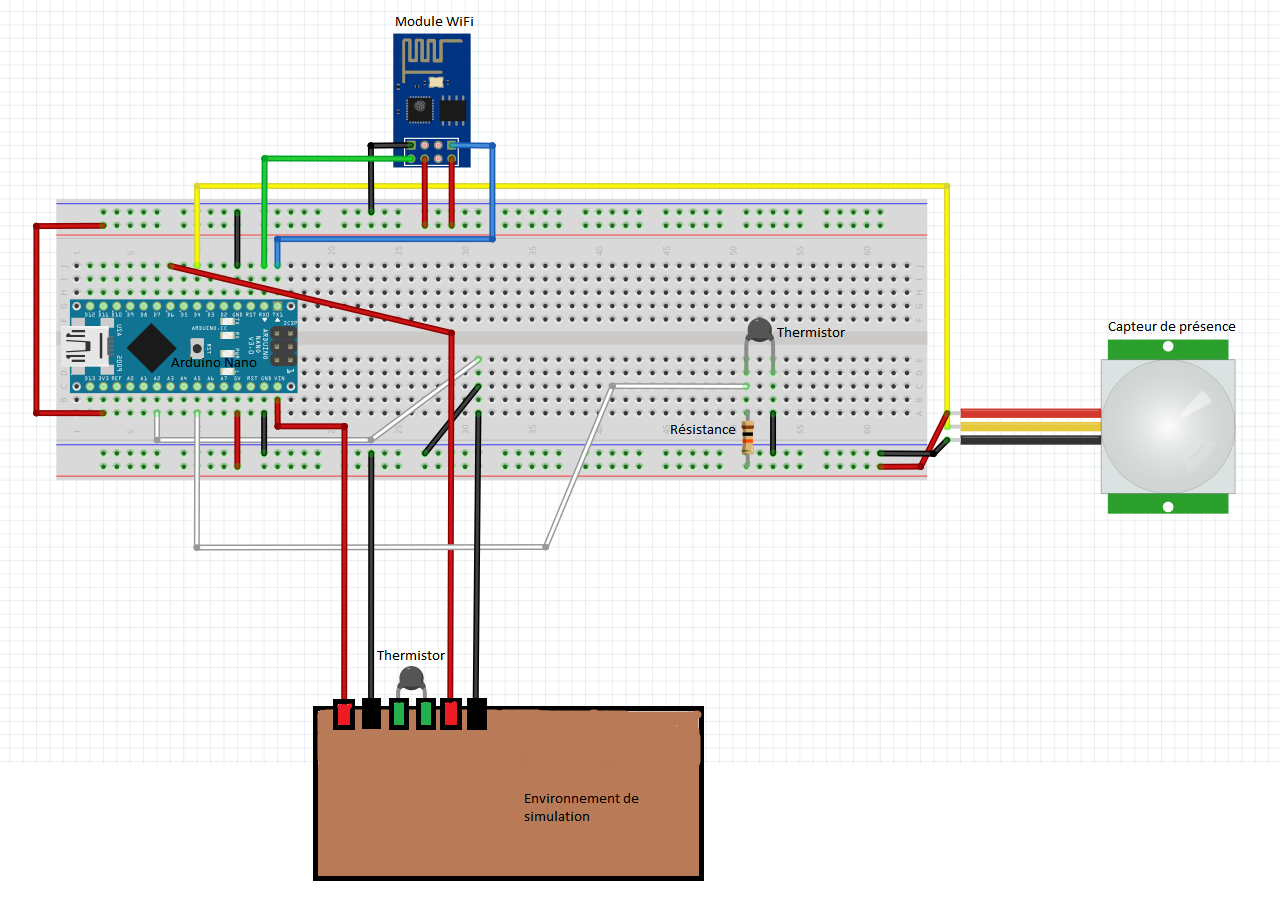
\includegraphics[scale=0.4]{cablage.PNG}
\caption{\label{cablage} Câblage de l'Arduino avec l'environnement de simulation}
\end{center}
\end{figure}

%Insérer des photo du prototype

\textbf{Instruction de montage:}
\begin{enumerate}
\item Brancher l'entrée RX du module WiFi avec la pin TX de l'Arduino ainsi que la sortie TX du module WiFi avec la pin RX de l'Arduino
\item Connecter le module WiFi à une source de tension de 3.3V et refermer le circuit en connectant la borne de sortie à la masse
\item Alimenter en 5V le capteur de présence et connecter le capteur à la masse
\item Connecter la 3ème entrée du capteur de présence à une pin digitale de l'Arduino
\item Brancher la thermistance en série avec la résistance de $10k\Omega$ et alimenter en 5V
\item Câbler la vanne (en PWM)
\item Câbler l'alimentation de l'Arduino
\end{enumerate}

\chapter{Contrôle et communication}
%Incorporer schéma de communication entre Arduino et Raspberry Pi
\section{Protocole de communication}
Afin de garantir une communication sans fil efficace entre l'unité centrale et les thermostats satellites, il nous a été demandé d'employer des requêtes HTTP \cite{_requests:_????} pour la transmission d'informations. Ces requêtes HTTP permettent différentes actions tel que l'enregistrement des thermostats individuels au sein de l'unité centrale, la transmission de donnée issues des différents capteurs ainsi que le contrôle de la vanne thermostatique. Dans le cadre de ce projet, nous avons eu recours à trois méthode HTTP: 

\begin{itemize}
\item PUT: lors de l'enregistrement 
\item GET: lors de la récolte des informations fournies par les capteurs
\item POST: lors de la mise en service de la vanne thermostatique
\end{itemize}

Dès l'initialisation d'un thermostat individuel, son adresses IP et son port sont envoyés à l'unité centrale, dont l'adresse IP est fixe, afin que ce dernier puisse ensuite les utiliser pour les interroger au moyen des requêtes HTTP.

\section{Rôle de l'unité centrale}
\subsection{Communication}
L'unité centrale a pour principal objectif la gestion de la communication avec les différents thermostats individuels. Elle se fait via un réseau Wifi qui a été préalablement configuré et la communication client-serveur respecte un protocole bien précis décrit dans la section précédente.
D'une part les thermostats satellites transmettent les informations récoltées par leurs différents capteurs, d'autre part l'unité centrale transmet les données nécessaires à la régulation du chauffage. Pour ce faire, le thermostat central doit être doté d'algorithmes de contrôle qui ont été implémentés en Python sur le Raspberry Pi. Les différents algorithmes de contrôles utilisés seront décrits en détail ultérieurement.\\

\noindent
La communication entre le thermostat central et les thermostats satellites (voir figure \ref{diagramme}) se fait de la manière suivante:\\

\begin{enumerate}
\item Tout d'abord l'unité centrale interroge chaque thermostat individuel au moyen d'une requête PUT et les invite à s'enregistrer dans sa base de données. C'est pourquoi chaque Arduino doit être configuré afin de pouvoir répondre à cette demande d'enregistrement. Il s'agit d'une tâche de fond qui s'exécute en permanence.\\
\item Une fois que les adresses IP et ports des thermostats individuels nous sont fournis lors de l'enregistrement de ces derniers, il nous suffit dès lors de les parcourir au moyen d'une boucle \emph{for} afin de toutes les consulter. Cependant une connexion doit au préalable être établie avec chaque thermostat. Pour ce faire, nous avons implémenté une classe \emph{Sensor} qui va garantir l'établissement de cette connexion grâce aux différentes méthodes de la librairie \emph{requests}. % références 
A chaque thermostat satellite est associé un objet de cette classe dont les méthodes vont permettre un accès en lecture (méthode \emph{get}) et en écriture (méthode \emph{set}) aux URL spécifiées. Concrètement, les accesseurs en lecture vont permettre à l'unité centrale de lire l'état des différents capteurs de chaque thermostat individuel tandis que les accesseurs en écriture vont permettre de modifier l'état de la vanne thermostatique.\\
\item Enfin, le thermostat central sonde chaque appareil enregistré et leur demande plusieurs informations telles que la température actuelle, le pourcentage d'utilisation de la vanne thermostatique et l'éventuelle détection d'une présence. Afin d'assurer une bonne gestion des informations captées, celles-ci transitent sur des chemins bien distincts: ce sont les URL.\\
Une URL est le chemin d'accès à une ressource du serveur questionné, elle présente une structure semblable à la suivante: \emph{protocole://adresse ip:port/ressource}\\
Le premier mot indique que la requête qui est faite au serveur respecte un protocole bien précis, dans notre cas il s'agit du protocole HTTP. Ensuite, il est nécessaire de spécifier l'appareil interrogé, ceci se fait en mentionnant son adresse IP ainsi que le port sur lequel il est connecté. Enfin tout ce qui s'ensuit représente le chemin d'accès à la ressource recherchée. Celle-ci peut contenir des informations enregistrées sous différents formats (HTML, text, JSON, etc). Par exemple, pour importer la température captée par un Arduino, il a fallu parcourir l'URL suivante: \emph{http://ip-arduino:port-arduino/temperature}\\ %m mettre en plus beau

\end{enumerate}
\noindent
\begin{figure}
\centering
\includegraphics[scale=0.3]{Diagram2.png}
\caption{\label{diagramme} Digramme de communication}
\end{figure}
De plus, afin d'assurer une communication simultanée entre l'unité centrale et les différents thermostats, nous avons utilisé le module \emph{threading} de Python qui va permettre au Raspberry Pi de communiquer avec tous les arduinos en même temps. Cette fonctionnalité voit son intérêt lorsque le nombre de thermostats satellites devient important. En effet, on peut aisément imaginer que plus ce nombre s'accroît, plus le temps de séparation entre deux sondages d'un même thermostat est long. Ceci peut devenir problématique dans le cadre d'une régulation qui nécessite une prise de onnaissance régulière de la température.

%nous avons importé la classe \emph{HTTPConnection} de la librairie \emph{http.client}\cite{http_protocol_client}. %mettre une référence de la doc python
%Cet objet instancie une connexion à l'adresse IP et au port spécifié. Il suffit dès lors d'envoyer une requête de type GET au chemin d'accès duquel on souhaite extraire des données. Cette opération instancie un objet de classe \emph{HTTPResponse} par lequel on peut accéder à toutes les informations demandées.\\%petit bout de code ?
% insérer un schéma ici (ou pas)

\subsection{Gestion des données}
L'unité centrale assure également le stockage de données, celles-ci sont utiles pour la prise de mesures expérimentales et l'implémentation d'algorithmes de contrôle intelligents se basant sur des données prélevées précédemment.\\
A ce stade, deux moyens de stockage d'informations se présentent:
\begin{itemize}
\item L'utilisation de fichiers
\item L'implémentation d'une base de données
\end{itemize}
Les fichiers sont faciles à utiliser et peuvent être modifiés manuellement en cas de besoin, cependant on ne peut pas enregistrer suffisamment de données dans un fichier.
Les bases de données ont beaucoup plus de capacité de stockage et présentent une structure de répartition par tables plus adaptée à la prise de mesures de données numériques. De plus, elles permettent une gestion des informations optimales grâce à ces fonctionnalités de tris de données. C'est pourquoi nous avons préféré la seconde option.
La base de données a été implémentée en utilisant \emph{SQLite} avec la bibliothèque \emph{sqlite3} de Python. Ce module est facile d'utilisation et a l'avantage d'être pré-installé sur Python. D'autres bases de données telles que \emph{MySQL} ou \emph{Oracle} auraient pu convenir mais elles ne présentaient pas de facilité d'accès de \emph{SQLite} \cite{_11.13._????}.\\

\noindent
La base de donnée a été implémentée de manière à assurer deux tâches:\\
\begin{itemize}
\item Elle va permettre d'une part le stockage des données de l'utilisateur. Ces données seront utiles à l'implémentation d'une intelligence artificielle se basant sur les statistiques de ce dernier. Cet aspect du projet est décrit en détail dans le chapitre \ref{intelligent}.\\ % mettre un lien c est mieux
\item D'autre part ces informations seront utilisées afin d'afficher les dernières données fournies par chaque thermostat dans une dashboard consultable par l'utilisateur depuis un navigateur web.
\end{itemize}

% dashboard

\subsection{Gestion des erreurs}
Afin de faciliter le codage de la communication du Raspberry Pi, celui-ci a d'abord été testé avec l'environnement de simulation, en effet celui ci a été fourni de telle sorte qu'il soit déjà opérationnel pour la communication sans fil avec notre prototype. Ainsi une éventuelle erreur de communication ne pouvait provenir que du code Python. En ce qui concerne les erreurs liées au code Python, elles ont été gérées grâce au couple d'instructions \emph{try-except}. Cette instruction a l'avantage de continuer l'exécution du programme malgré la survenance d'une erreur dans l'algorithme de contrôle. La commande \emph{except} permet de sauter les lignes de code sujet à erreur et d'exécuter ce qui suit ce mot clef. Dans notre situation, la majorité des erreurs apparaissent lors de l'exécution de requêtes. En effet, le matériel utilisé dans ce projet ne permet pas une communication optimale entre l'unité centrale et les thermostats satellites. Afin de gérer ces erreurs nous avons opté pour la mise en place d'un système de timeout directement disponible à partir de la fonction \emph{get} du module \emph{requests}: Si la requête ne s'effectue pas avant un certain nombre de secondes, celle-ci renvoie \emph{None} et l'exécution du code reprend son cours.

\chapter{R\'{e}gulation de la température}
Le but du projet \'{e}tant de pouvoir chauffer une  pi\`{e}ce, il est donc important de pouvoir générer un alogrithme de contr\^{o}le accomplissant cette t\^{a}che. Ce dernier sera impl\'{e}ment\'{e} dans le thermostat central et via le protocole de communication ,des ordres pourront être envoy\'{e}s aux thermostats individuels. Une fois les commandes reçues, la vanne pourra \^etre actionn\'{e}e selon la temp\'{e}rature de consigne de la zone. 
L'impl\'ementation de l'algorithme de contr\^ole se d\'eroule en plusieurs \'{e}tapes. Il s'agit de mettre en place un codage bas\'{e} sur une d\'etection r\'eactive. Pour ce faire, nous d\'{e}butons avec une r\'{e}gulation on/off suivie de l'\'{e}tude de la conception d'un P.I.D.

\section{Régulation ON/OFF}
La r\'{e}gulation on/off est une simple m\'{e}thode permettant d'actionner la vanne à 100\% dans le cas o\`{u} la temp\'{e}rature ambiante est en dessous de la temp\'{e}rature de consigne . Elle d\'{e}sactive l'ouverture de la vanne lorsque la température ambiante vaut ou dépasse la consigne.\\
Voici l'allure des courbes de température obtenues lors de nos expériences (figure \ref{onoff}):

\begin{center}
\begin{figure}[H]
    \begin{minipage}[t]{8cm}
        \centering
        \subfigure[consigne = 25°C]{\label{plan1}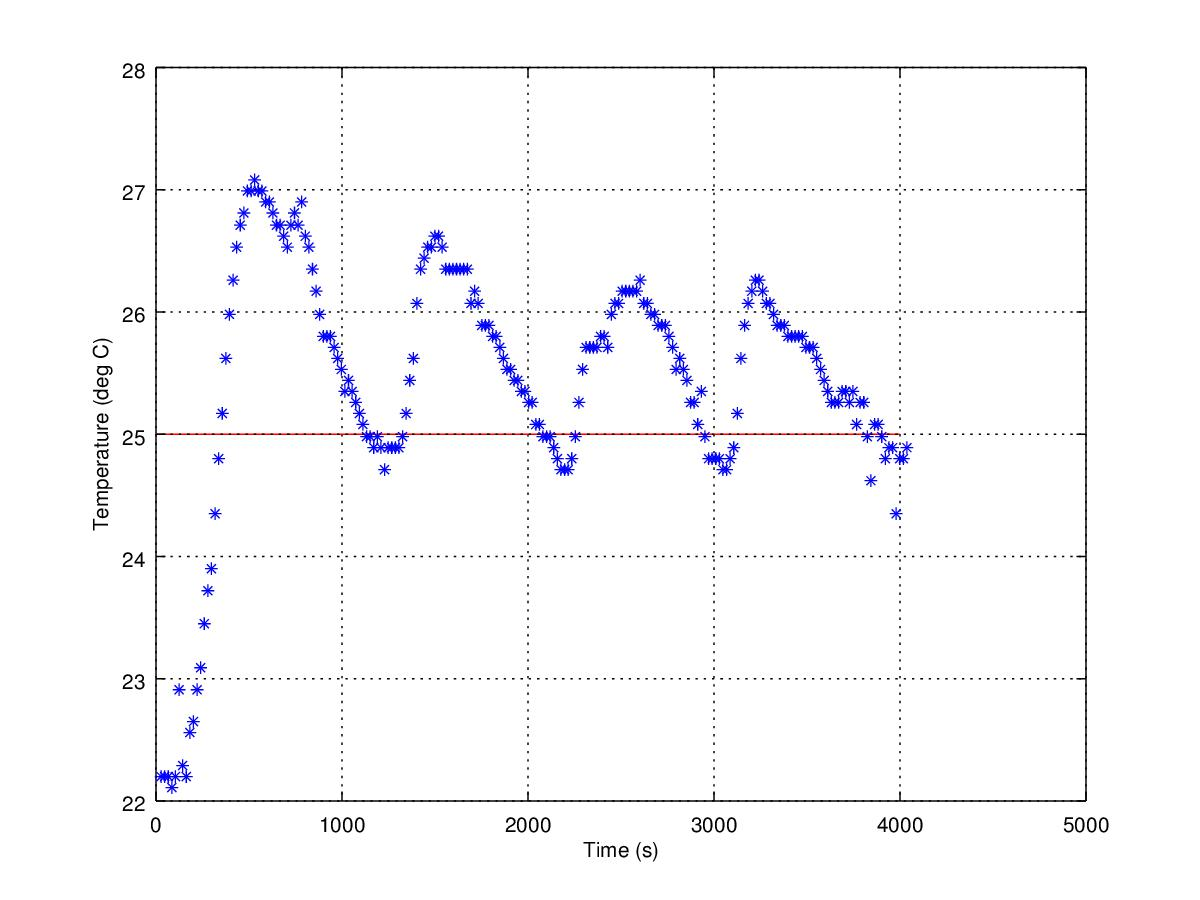
\includegraphics[width=8cm]{pc24.jpg}}
    \end{minipage}\hfill
    \begin{minipage}[t]{8cm}
        \centering
        \subfigure[consigne = 30°C]{\label{plan2}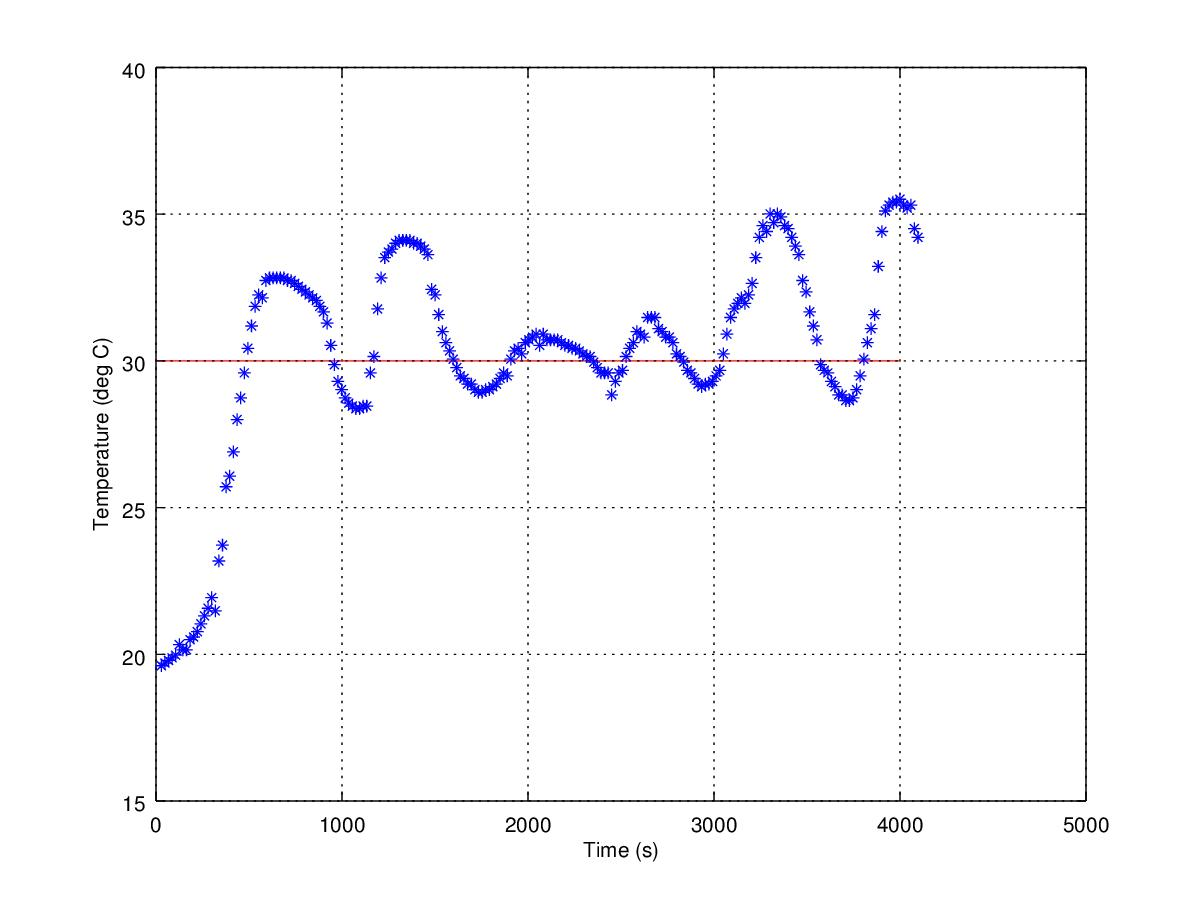
\includegraphics[width=8cm]{onoff30.jpg}}
    \end{minipage}
    \caption{\label{onoff} Mesures pour l'algorithme On/Off pour différentes températures de consigne}
\end{figure}
\end{center}

Sur ces graphes, on observe de fortes oscillations autour de la température de consigne. Cela est dû au fait que le syst\`{e}me a une inertie dont l'algorithme on/off ne tient pas compte. Ce phénomène est fortement visible sur la courbe verte de la figure 5.1. Dès que la température de consigne est dépassée, la vanne va à 0 mais l'inertie du système fait que la température continue quand même à augmenter.


\section{Régulation PID}
%Il se trouve que lorsque la temp\'{e}rature de la zone atteint la temp\'erature de consigne, la vanne se ferme. Seulement la temp\'erature ne se stabilise pas et elle diminue car il ne faut pas oublier de tenir compte des perditions ainsi que de la temp\'erature ext\'erieure. L'écart se diff\`ere de z\'ero et ainsi la vanne est activ\'ee. Ce processus draconien n'est pas des plus efficaces car il userait la vanne. En effet, il suffit que la diffe\'rence de temp\'erature soit minime (0,5°) pour que la vanne passe de "marche" à "arr\^et" puis "marche"... et le cycle se perp\'etue .\\
\subsection{Généralités}
La régulation P.I.D tente d'approcher la valeur de consigne au plus juste tout en faisant en sorte que les pertes de chaleur de la zone à chauffer soient compens\'{e}es en analysant régulièrement le système et en ajustant systématiquement la commande en fonction de la valeur de consigne (voir figure \ref{regulateur}).\\
\noindent
La m\'{e}thode PID (proportionnel, int\'egrale, d\'eriv\'ee) se d\'{e}compose en 3 fonctions (f\ref{eq1}). Tout d'abord, la partie proportionnelle qui d\'{e}pend de l'\'{e}cart de temp\'{e}rature entre la température ambiante et la consigne. Cet \'{e}cart portera le nom d'erreur. En effet, plus l'erreur est grande plus le pourcentage d'ouverture de la vanne augmente. Consid\'{e}rons une consigne fix\'{e}e \`{a} 20°C et une temp\'{e}rature ambiante de 15°C, la vanne est en premier lieu activ\'{e}e \`{a} 100\%. Seulement, lorsque l'erreur diminue et que la temp\'{e}rature est \`{a} 19°C, la vanne n'est ouverte plus qu'\`{a} 30\%. Le but n'étant de jamais vraiment atteindre la valeur consigne car si la vanne se ferme la température baisse. Dans la formule, l'erreur est multipli\'{e}e par un coefficient Kp.\\ %Le coefficient de proportionnalit\'{e} se d\'{e}termine empiriquement.

\noindent
La seconde branche de l'\'{e}quation est une int\'{e}grale qui consiste \`{a} faire la somme des erreurs au cours du temps. Plus on chauffe, plus l'erreur globale augmente et plus on continue de chauffer. Mais dans le cas o\`{u} la temp\'{e}rature d\'{e}passe la consigne, l'erreur globale diminue ce qui permet de d\'{e}c\'{e}l\'{e}rer la commande. Cette composante est additionn\'{e}e à la partie proportionnelle car elle permet de pouvoir annuler l'erreur restante (due \`{a} la composante proportionnelle) de sorte \`{a} ce que la temp\'{e}rature soit \'{e}gale \`{a} la consigne.\\

\noindent
La derni\`{e}re composante est une d\'{e}riv\'{e}e. Elle peut se calculer en consid\'{e}rant l'erreur courante et l'erreur pr\'{e}c\'{e}dente divis\'{e}es par le temps s\'{e}parant ces deux erreurs. Le but de cette d\'{e}riv\'{e}e est de pouvoir freiner la commande dans le cas o\`{u} l'augmentation de temp\'{e}rature est trop rapide. Ceci permettra de pouvoir atteindre au mieux la valeur consigne en \'{e}vitant le plus d'oscillations possibles.\\

\begin{figure}[H]
\centering
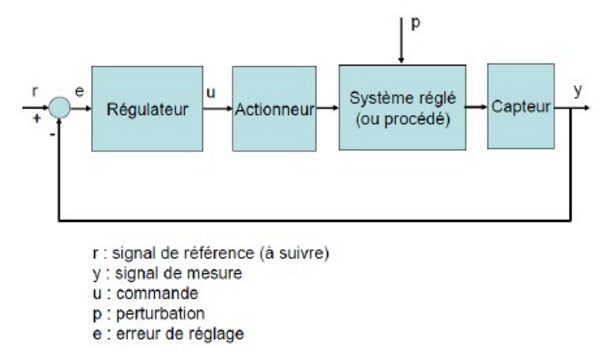
\includegraphics[scale = 0.8]{Regulateur.PNG}
\caption{\label{regulateur} Schéma régulation présenté lors du séminaire de Laurent Catoire}
\end{figure}

\begin{equation}
CO = Kp \cdot erreur(t) + Ki \cdot\ \int_{ti}^{tf}  erreur(t) \, \mathrm dt + Kd \cdot \frac{derreur(t)}{dt}
\label{eq1}
\end{equation}
où \emph{ CO = commande (pourcentage d'ouverture de la vanne)}\\

%Pour pouvoir se procurer les coefficients Kp, Ki, Kd de l'\'equation, des s\'{e}ries de tests doivent \^{e}tre r\'{e}alis\'{e}s comprenant des graphes \'{e}tudiant l'\'{e}volution, au cours du temps, de la temp\'{e}rature par rapport \`{a} la consigne.\\
%Ce mod\`{e}le sera mis en pratique lors du second quadrimestre.

Ce modèle est beaucoup plus rigoureux que le précédent. Son avantage réside dans le fait qu'il assure une régulation sans pour autant imposer la connaissance des paramètres physiques du système.
Cependant il faut encore déterminer les trois constantes \emph{Kp, Ki et Kd}: Celles-ci peuvent se trouver expérimentalement. La principale difficulté de l'implémentation du régulateur PID est le fait que les constantes varient en fonction des différents paramètres physiques du système comme la conductivité thermique du matériau isolant, la température initiale de la pièce, etc. Ainsi les constantes \emph{Kp, Ki, Kd} ne sont pas vraiment des constantes dans le sens où elles n'auront pas forcément les mêmes valeurs d'une période de la journée à une autre ou d'un milieu expérimental à un autre.\\
Il est donc nécessaire d'introduire à notre algorithme de régulation une phase de calibration dont le but sera de déterminer les valeurs des 3 constantes. Pour ce faire, nous avons eu recours à la méthode de Ziegler-Nichols\cite{_commande_????}. Celle-ci est décrite dans la section suivante.\\

\subsection{Calibration}
La méthode de Ziegler-Nichols est une méthode graphique qui consiste à maintenir la vanne allumée à une valeur constante pendant un intervalle de temps suffisamment long. Une fois la courbe de l'évolution de la température en fonction du temps obtenue, il suffit de trouver le point présentant la plus grande pente. La courbe obtenue après ce processus est semblable à la suivante: \ref{graphe2}:\\

\begin{figure}[H]
\begin{center}
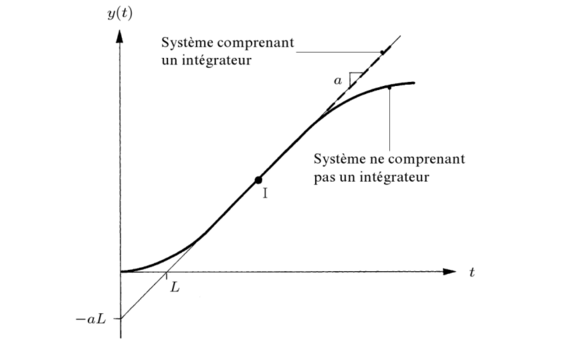
\includegraphics[scale = 0.95]{zn.PNG}
\caption{\label{graphe2} Méthode de Ziegler-Nichols en théorie tirée de l'ouvrage: \cite{_commande_????}}
\end{center}
\end{figure}

Après avoir trouvé ce point particulier (il s'agit du point \emph{I}), il suffit de trouver le point d'intersection des droites suivantes:\\
\[\left\{ 
\begin{array}{l l}
y(t) = y_{I} + a (t-t_{I})\\
y(t) = T_{0}\\ 
\end{array} 
\right. \]
où:  \begin{itemize}
\item $y(t)$ représente la température en fonction du temps
\item $T_{0}$ représente la température initiale du processus de chauffe (il s'agit de l'axe des abscisses dans la figure \ref{graphe2})
\item $a$ est la plus grande pente du graphique pondérée par la valeur de la vanne (comprise entre 0 et 100)
\end{itemize}
La solution de ce système d'équations nous renseigne sur le point $L$ qui représente le temps de réaction de chauffage due à l'inertie du système. Une fois les variables $a$ et $L$ trouvées, Ziegler-Nichols nous proposent des formules dépendantes de ces deux paramètres qui nous permettront de déterminer les constantes \emph{Kp, Ki et Kd}. Cependant nous nous sommes permis d'adapter ces formules aux expériences faites sur notre prototype compte-tenu de la nature empirique de ces relations. Les valeurs obtenues sont représentées dans le tableau \ref{tab1}.\\
\begin{table}
\begin{center}
\begin{tabular}{|m{2cm}|m{1cm}|m{1cm}|m{1cm}|}
\hline
 &$K_p$&$K_i$&$K_d$\\
\hline
\vspace{0.5cm}
  {PID}&{$\frac{12}{aL}$}&{$\frac{100\cdot K_p}{2\cdot L}$}&{$\frac{K_p \cdot L}{2000}$}\\
\hline
\end{tabular}
\caption{\label{tab1} Tableau des constantes du PID}
\end{center}
\end{table}\\

En pratique, lors de la phase de calibration, nous utilisons l'analyse numérique afin de déterminer le point \emph{I}. En effet il suffit de se rappeler que:\\
\begin{equation}
\frac{dy_{i}}{dt} = \frac{y_{i+1} - y_{i-1}}{2\cdot h} + O(h^2)
\end{equation}
\begin{equation}
a = max(\frac{dy_i}{dt})
\end{equation}
où 
\emph{h} est le pas d'intégration, typiquement il s'agit du temps séparant la mesure \emph{i} et \emph{i+1}.\\

Cependant cette méthode présente quelques inconvénients:
\begin{itemize}
\item La phase de calibration peut durer de 15 à 20 minutes.
\item La méthode utilisée est très sensible au bruit de mesures. Ceci est illustré dans la figure \ref{graphe4}. On observe que l'allure de la courbe de calibration que nous avons obtenu est la même que celle présentée théoriquement, néanmoins on peut remarquer la présence de mesures dites parasites situées en dehors de la courbe. A premier abord, ceci paraît négligeable, toutefois on remarque que ces bruits de mesures peuvent perturber grandement les valeurs des constantes lorsque l'on analyse les équations (5.2) et (5.3). En effet, le point du graphique présentant la plus grande pente sera probablement un point situé au voisinage de ces mesures parasites alors que ce n'est pas forcément le cas.\\
Afin d'éviter ce phénomène, nous avons dû implémenté un algorithme qui détecte les valeurs aberrantes de la série statistique obtenue. Ce-dernier éliminera tous les points dont l'accroissement est supérieur à une valeur limite définie arbitrairement.
\end{itemize}

\begin{figure}
\begin{center}
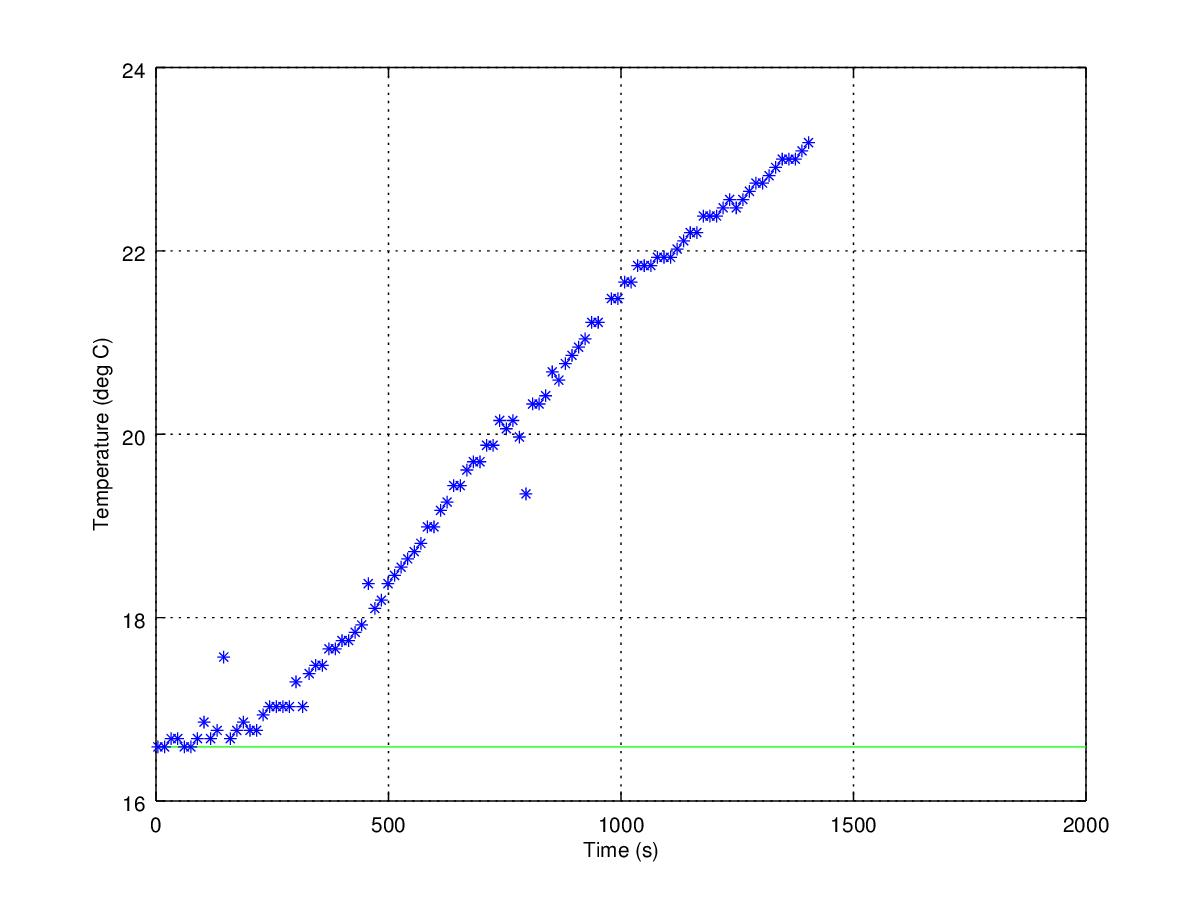
\includegraphics[scale = 0.6]{vanne40.jpg}
\caption{\label{graphe4} Méthode de Ziegler-Nichols en pratique}
\end{center}
\end{figure}
\noindent
Une fois les constantes déterminées, on s'attend à obtenir une courbe de la régulation PID semblable à celle représentée sur la figure \ref{graphe3}.\\
Les courbes obtenues expérimentalement (voir figure \ref{pid}) ont une allure proche de celle recherchée.

\begin{figure}
\begin{center}
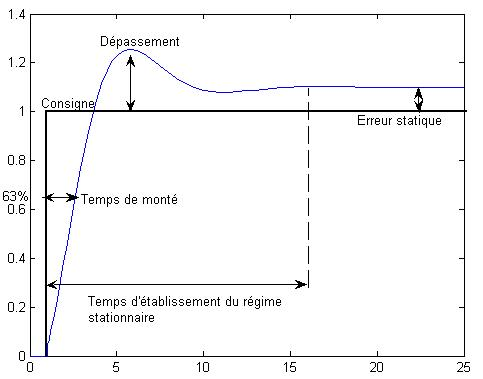
\includegraphics[scale = 0.85]{Reponse_echelon_PID.png}
\caption{\label{graphe3} P.I.D: Image tir\'{e}e de Wikip\'{e}dia}
\end{center}
\end{figure}

\begin{center}
\begin{figure}[H]
    \begin{minipage}[t]{8cm}
        \centering
        \subfigure[consigne = 25°C]{\label{plan3}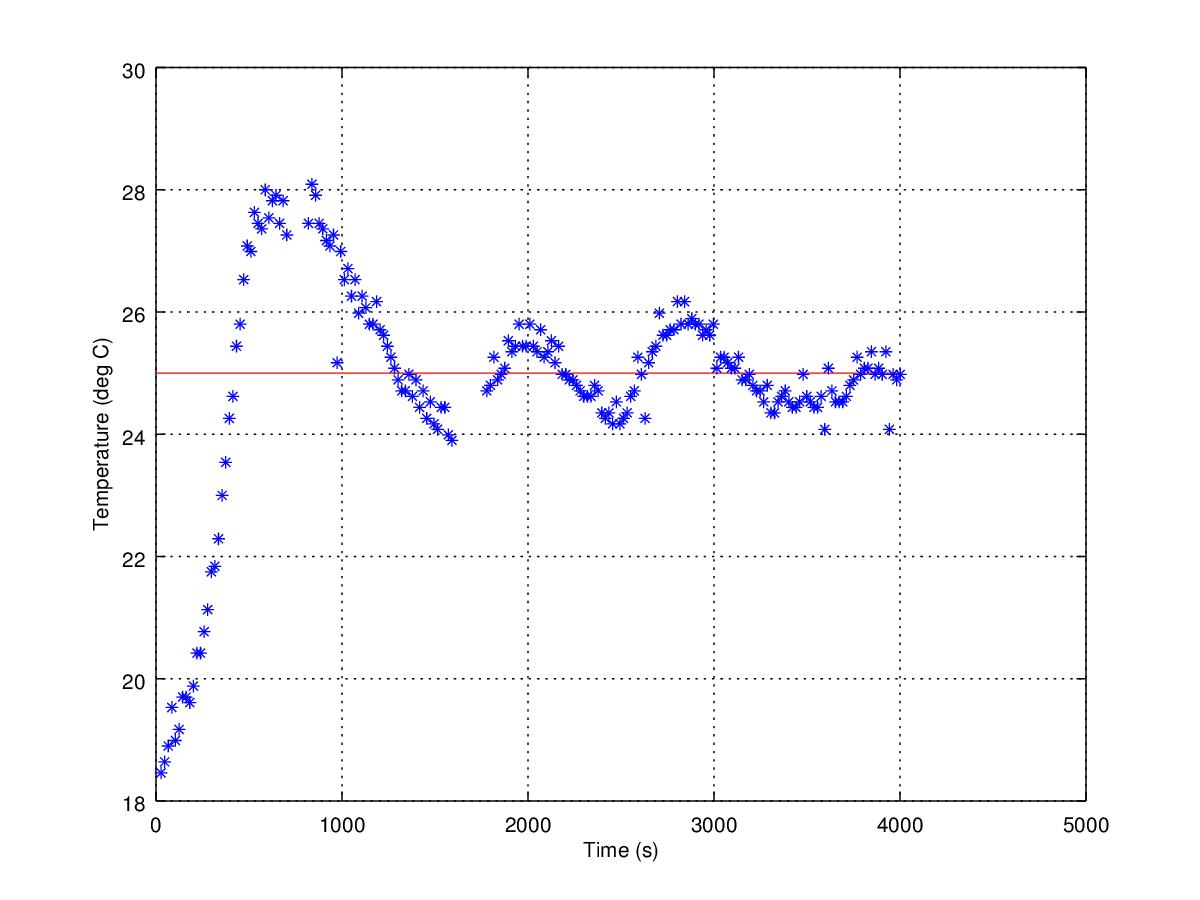
\includegraphics[width=8cm]{pid25.jpg}}\\
        $K_p = 26.76$, $K_i = 1.16$, $K_d = 15.42$
    \end{minipage}\hfill
    \begin{minipage}[t]{8cm}
        \centering
        \subfigure[consigne = 30°C]{\label{plan4}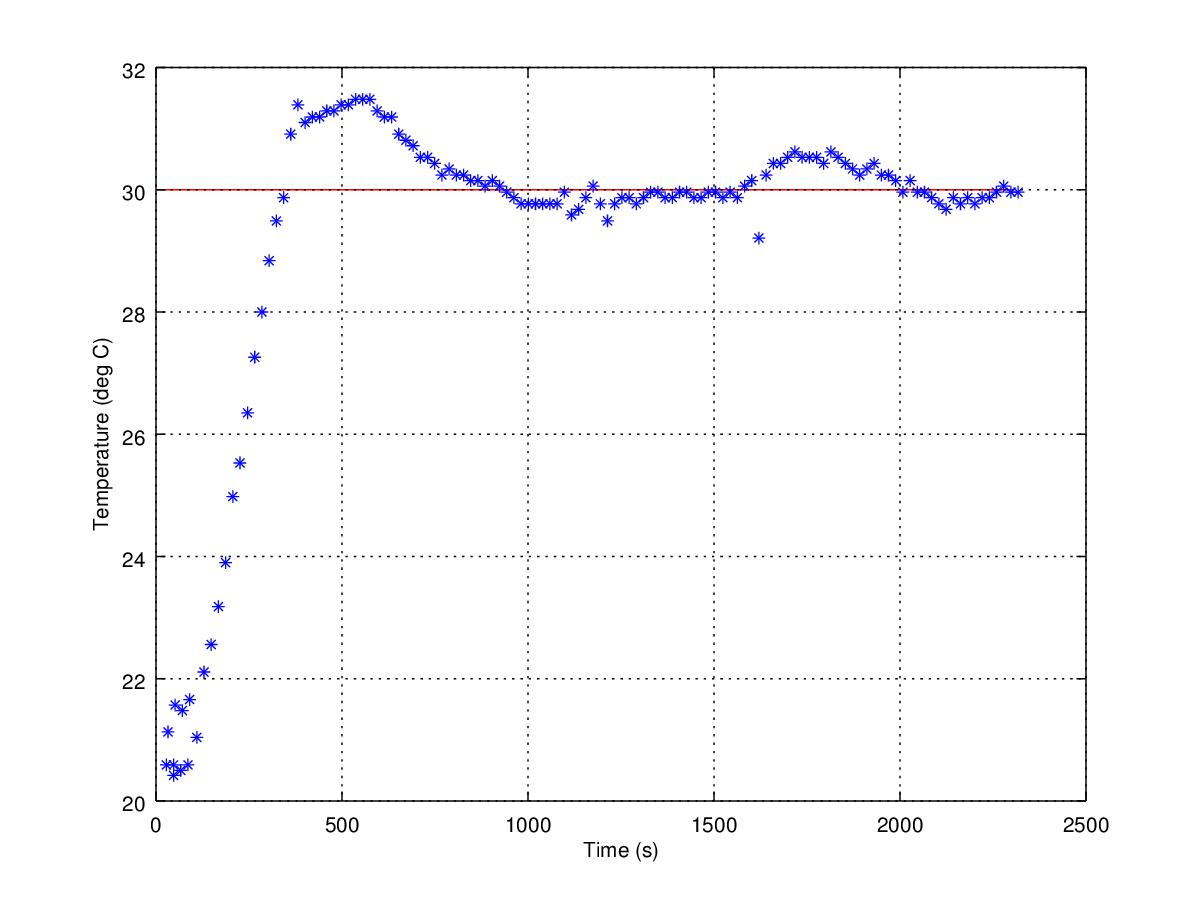
\includegraphics[width=8cm]{pc5.jpg}}\\
        $K_p = 11.37$, $K_i = 0.59$, $K_d = 5.5$
    \end{minipage}
    \caption{\label{pid} Mesures du PID pour différentes températures de consigne}
\end{figure}
\end{center}

\section{Indices de qualité}

Après avoir discuté les différents algorithmes implémentés pour la régulation de la température, il est nécessaire d'introduire un indice de qualité. Il s'agit d'un nombre compris entre 0 et 1 qui jugera l'efficacité de l'algorithme implémenté. Différents facteurs seront pris en compte lors de l'évaluation des différentes méthodes de régulation, à savoir:
\begin{enumerate}
\item La vitesse à laquelle la température atteint sa valeur de consigne
\item La consommation d'énergie du chauffage
\item L'amplitude moyenne des oscillations autour de la température de consigne
\end{enumerate}

\noindent
Une fois les critères d'évaluation de l'algorithme établis, il est naturel de leur attribuer une pondération qui les classera par ordre d'importance, ce choix est tout à fait arbitraire, d'ailleurs les critères mentionnés ci-dessus le sont également.\\
Nous avons décidé de pondérer chaque point de la manière suivante:
\begin{equation}
i = \frac{1}{6} \cdot c_1 + \frac{1}{2} \cdot c_2 + \frac{1}{3} \cdot c_3
\label{indice}
\end{equation}
où:
\begin{itemize}
\item $i$ est l'indice de qualité avec: $0 \le i \le 1$ 
\item $c_1, c_2, c_3$ sont les trois critères d'évaluation cités ci-dessus avec: $0 \le c_k \le 1 (k= 1,2,3)$
\end{itemize}

\subsection{Critère n°1: Temps d'atteinte de la température de consigne}
Afin de définir le niveau de vitesse de chauffage, il est nécessaire d'introduire une valeur de celle-ci que l'on considérera comme optimale. Il s'agit d'une valeur qui ne peut être atteinte que si la vanne est allumée à 100\% dès le début de l'expérience. Il est à noter que les valeurs obtenues ne sont cohérentes que si les différentes mesures sont effectuées dans de même conditions expérimentales.\\
On définit alors:
\begin{equation}
c_1 = \frac{temps_{optimal}}{temps_{mesure}}
\end{equation}

\noindent
Compte tenu de la définition du temps optimal, on déduit aisément que, pour l'algorithme \emph{On/Off}, $c_1 = 1$, c'est-à-dire la valeur maximale.\\
\noindent
Les graphes ci-dessous (\ref{comp1}) représentent les temps mis par chaque algorithme pour atteindre la température de consigne:

\begin{center}
\begin{figure}[H]
    \begin{minipage}[t]{8cm}
        \centering
        \subfigure[PID]{\label{plan5}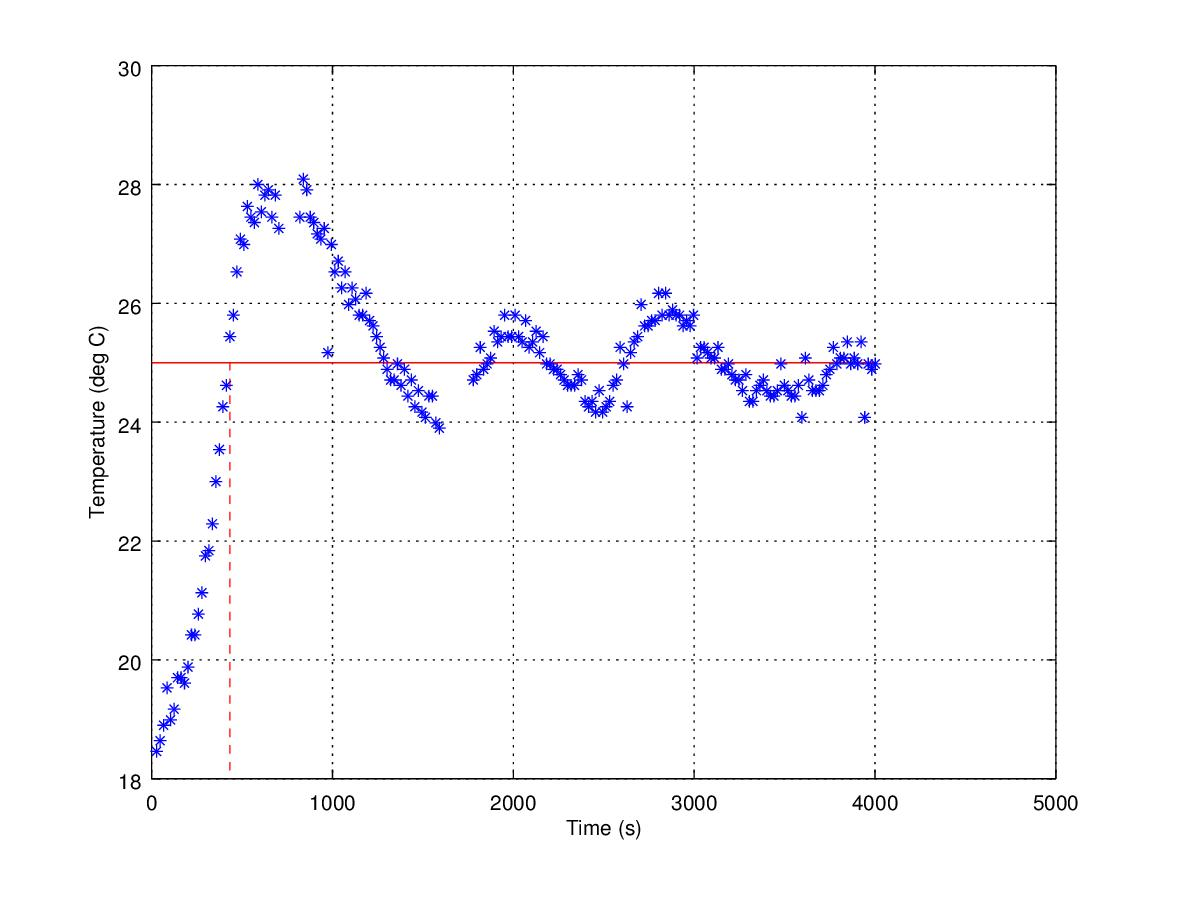
\includegraphics[width=8cm]{c1_pid.jpg}}
    \end{minipage}\hfill
    \begin{minipage}[t]{8cm}
        \centering
        \subfigure[On/Off]{\label{plan6}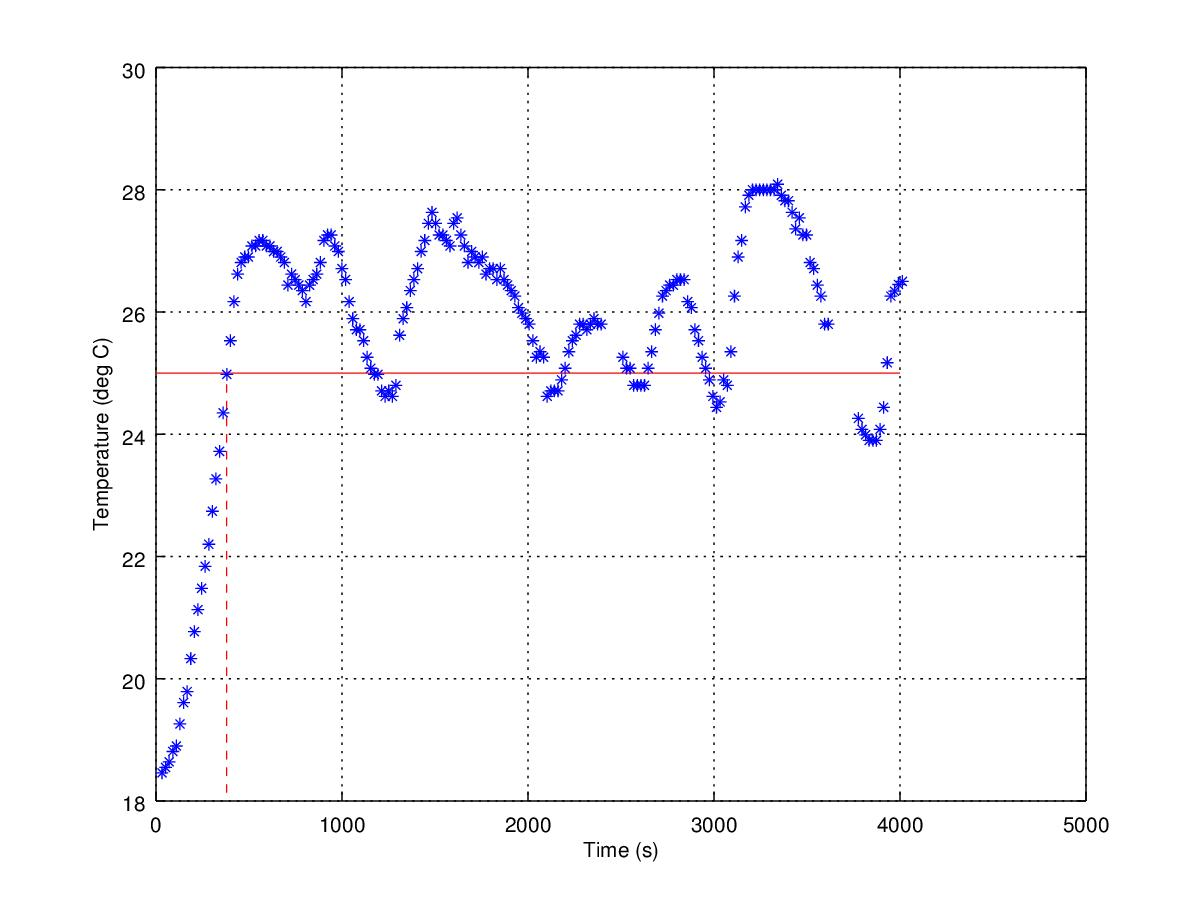
\includegraphics[width=8cm]{comp.jpg}}
    \end{minipage}
    \caption{\label{comp1} Graphes de comparaison entre la régulation on/off et PID}
\end{figure}
\end{center}

On constate comme attendu que le régulateur On/Off est plus rapide que le PID. En effet, on obtient un temps de 432 secondes pour le PID contre 380 secondes pour le second. On a alors compte tenu de l'équation (5.5):
\[\left\{ 
\begin{array}{l l}
c_{1, on/off} = 1 \\
c_{1, pid} = \frac{380}{432} \approx 0.88\\ 
\end{array} 
\right. \]

\subsection{Critère n°2: Consommation d'énergie}
Un autre critère que nous jugeons pertinent pour l'évaluation de nos algorithmes de chauffage est l'énergie totale consommée après chaque processus de chauffe. A priori ce critère n'est pas facile à déterminer car il dépend de plusieurs paramètres physiques comme illustré dans la formule ci-dessous:
\begin{equation}
Q_i = m\cdot C_p \cdot (T_i-T_0)
\end{equation}
Cependant on peut aisément s'affranchir des paramètres physiques $m$ et $C_p$ car les milieux expérimentaux restent les mêmes d'une expérience à l'autre. Ainsi, ces constantes physiques propres aux conditions expérimentales ne seront plus objets à comparaison.\\
Toutefois il est utile de se rappeler que l'énergie dissipée est proportionnelle à la différence entre la température à la $i^{eme}$ itération $T_i$ et la température initiale $T_0$. De plus, en se rappelant que:
\begin{equation}
Q = \sum_{i}Q_i
\end{equation}
on peut aisément ramener la comparaison de l'énergie dissipée de nos deux algorithmes à celle de l'aire sous la courbe de chacun de leur graphe.\\
Afin de déterminer l'aire sous la courbe de chaque graphe, nous avons eu recours à la méthode des trapèzes. Celle-ci consiste à découper le graphique en de nombreux trapèzes arbitrairement petits. La somme des aires de chaque trapèze approxime alors assez bien l'aire sous la courbe étudiée.\\

\noindent
En outre il est nécessaire d'introduire une aire dite optimale pour faciliter la définition du critère $c_2$. Celle-ci sera l'aire du rectangle défini ci-dessous:\\
\begin{equation}
\label{aire}
Aire_{optimale} = (t_{fin} - t_{montee})\cdot(T_{consigne} - T_0)
\end{equation}
où:
\begin{itemize}
\item $t_{montee}$ et $t_{fin}$ sont respectivement le temps optimal de montée jusqu'à la température de consigne $T_{consigne}$ et le temps total de l'expérience
\item $T_0$ est la température initiale à laquelle débute l'expérience
\end{itemize}
\noindent
Similairement au critère $c_1$, on définira le second critère de la façon suivante:\\
\begin{equation}
c_2 = \frac{Aire_{optimal}}{Aire_{mesure}}
\end{equation}
Où $Aire_{optimal}$ est déjà connue, elle vaut d'après sa définition (\ref{aire}):
\begin{equation}
Aire_{optimale} = (4000 - 380)\cdot(25 - 18.5) = 23530
\end{equation}
Voici les aires obtenues pour les deux algorithmes étudiés, il s'agit de la surface délimitée en jaune dans les graphes \ref{comp2}
\[\left\{ 
\begin{array}{l l}
Aire_{pid} = 25652 \\
Aire_{on/off} = 28700\\ 
\end{array} 
\right. \]
\noindent
Nous obtenons ainsi les valeurs suivantes pour le second critère:
\[\left\{ 
\begin{array}{l l}
c_{2, pid} = \frac{23530}{25652} \approx 0.92\\
c_{2, on/off} = \frac{23530}{28700} \approx 0.82\\ 
\end{array} 
\right. \]

\begin{center}
\begin{figure}[H]
    \begin{minipage}[t]{8cm}
        \centering
        \subfigure[PID]{\label{plan7}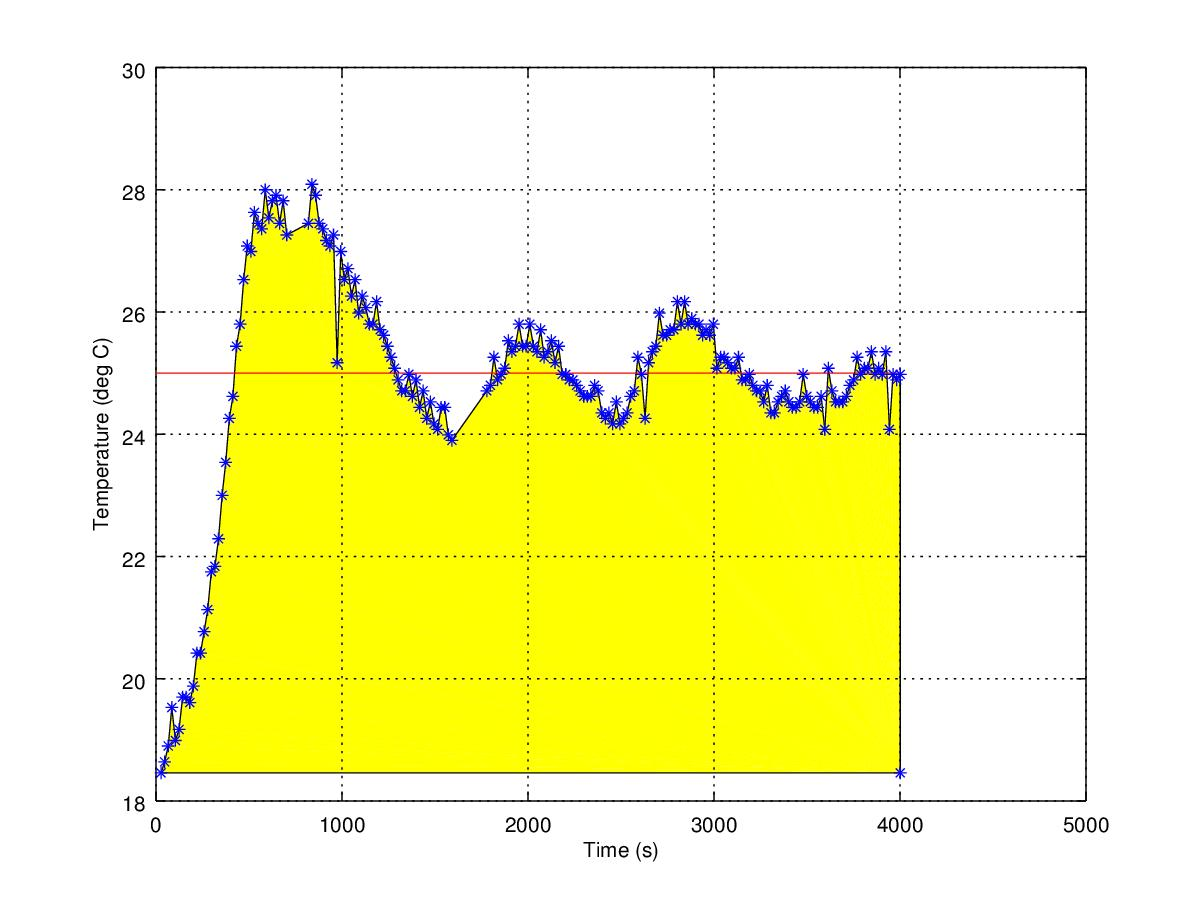
\includegraphics[width=8cm]{aire_pid.jpg}}
    \end{minipage}\hfill
    \begin{minipage}[t]{8cm}
        \centering
        \subfigure[On/Off]{\label{plan8}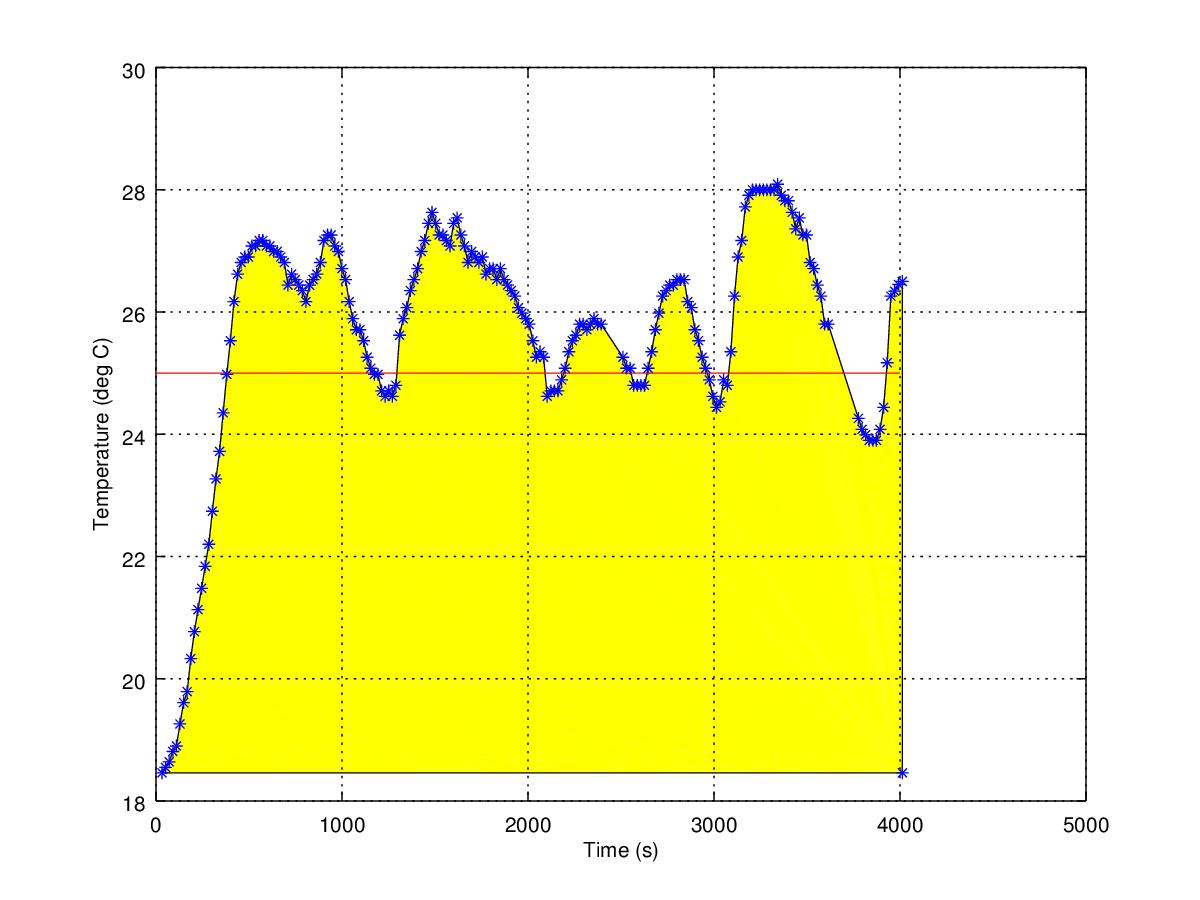
\includegraphics[width=8cm]{aire_onoff.jpg}}
    \end{minipage}
    \caption{\label{comp2} Graphes de comparaison entre la régulation On/Off et PID}
\end{figure}
\end{center}

\subsection{Critère n°3: Amplitude des oscillations}
Notre dernier critère d'évaluation consiste à mesurer la stabilité de chaque algorithme de régulation. Pour ce faire nous calculons la somme des amplitudes des oscillations de la température autour de la valeur de consigne. Plus l'amplitude sera faible, plus la valeur de $c_3$ sera proche de 1. A contrario une grande valeur de cette amplitude sera synonyme d'instabilité et $c_3$ se rapprochera de 0. Voici la définition choisie du troisième critère de comparaison:\\
\begin{equation}
c_3 = \frac{1}{|1+ amplitude|}
\label{c3}
\end{equation}
\noindent
La valeur absolue intervenant dans la formule (\ref{c3}) assure que l'amplitude sera positive (une amplitude peut être négative si l'oscillation se fait en-dessous de la valeur de consigne). Des trois critères discutés jusqu'à présent, il s'agit du plus exigent car il présente de faibles valeurs pour les deux algorithmes.\\
\noindent
Les résultats obtenus pour ce dernier critère de comparaison sont les suivants:
\[\left\{ 
\begin{array}{l l}
c_{3, pid} = \frac{1}{|1+2.47|} \approx 0.29\\
c_{3, on/off} = \frac{1}{|1+9.28|} \approx 0.1\\ 
\end{array}
\right. \]

\subsection{Résultats}

Après avoir calculé nos différents critères de comparaison, nous pouvons en déduire la valeur des indices de qualité pour chaque algorithme de régulation. En appliquant la formule (\ref{indice}), on obtient les valeurs suivantes:
\[\left\{ 
\begin{array}{l l}
i_{pid} \approx 0.7\\
i_{on/off} \approx 0.61\\
\end{array}
\right. \]
On constate que la régulation PID est plus performante que la régulation On/Off. Cependant, comme mentionné précédemment, l'indice de qualité introduit tout le long de ce chapitre n'est pas absolu. 

%courbe calculant l'inertie de l'environnement  : (la courbe peut depasser la valeur consigne meme en on/off) (voir figure \ref{graphe2})

%\begin{figure}
%\begin{center}
%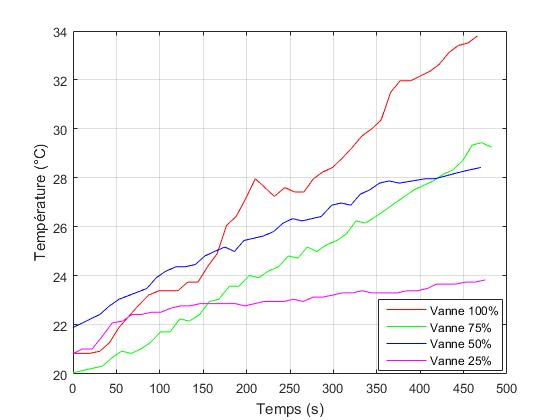
\includegraphics[scale = 0.65]{graphe2.jpg}
%\caption{\label{graphe2} Graphe évolution de la T° avec vanne à plusieurs niveaux}
%\end{center}
%\end{figure} 

\chapter{\label{intelligent}Thermostat intelligent}
%WWW pour le contrôle à distance
%Application smartphone
%Notification demande de préchauffement
%Géolocalisation
%Apprentissage comportement
%Pièces exploitées le plus souvent
%Choper information de la météo
%Système de surveillance via le module caméra du Raspberry Pi
\section{Gestion automatique de la température et prévision des heures d'utilisation} 
Afin d’améliorer l'utilisation du thermostat intelligent, il a été nécessaire d’élaborer un algorithme permettant de déterminer les fréquences d'utilisation de ce dernier afin d’en anticiper son usage.\\

\noindent
L’algorithme en question doit être capable de sauvegarder les données obtenues par les capteurs individuels. L’utilisation de fichiers a été choisie pour enregistrer et modifier ces informations. L’exploitation des bases de données ainsi constituées pourrait servir à la sauvegarde de telles informations, cependant le module sqlite3 nécessite quelques connaissances du langage SQL.
De plus, les bases de données générées par sqlite3 sont destinées à l’enregistrement d’un grand nombre de données permettant de créer un tableau de bord sur le web.\\

\noindent
Nous nous servons d’un dictionnaire dont les clés sont constituées de tuples. Les éléments de ces tuples reprennent le nom de l’arduino transmettant les informations et le jour de la semaine correspondant au jour de transmission de ces informations par l’arduino. Les valeurs associées à ces clés constituent des listes dont les éléments sont également des listes.\\

\noindent
Pour concevoir ce programme d'intelligence artificielle, il a été nécessaire de séparer une journée en tranches de 10 minutes soit en 144 parties. En utilisant ces 144 tranches, des listes de 6 éléments sont générées. Dans l’ordre, ces éléments s'énumèrent comme suit : le numéro du jour de la semaine (allant de 0 à 6, le chiffre 0 correspondant au lundi), le numéro du jour de l’année, l’année, l’heure, le nombre de minutes, le nombre de passages de « False » à « True » en suite de la détection d'une présence et enfin le nombre de semaines écoulées reprenant l’analyse des habitudes de l’utilisateur. Il y a donc 144 listes rassemblées en une seule pour chaque arduino actif et ce pour chaque jour de la semaine.\\

\noindent
On peut illustrer la création d'un tel fichier grâce à un tableau dont les colonnes représentent les arduino connectés et les rangées reprennent les jours de la semaine.
\vspace{0.2cm}
\begin{center}
\begin{tabular}{|c|c|c|c|c|c|}
\hline
{}&{arduino1}&{arduino2}&{arduino3}&{arduino4}&{arduino5}\\
\hline
{Lundi}&{liste1}&{...}&{...}&{...}&{liste5}\\
\hline
{Mardi}&{liste6}&{...}&{...}&{...}&{...}\\
\hline
{Mercredi}&{...}&{...}&{...}&{...}&{...}\\
\hline
{Jeudi}&{...}&{...}&{...}&{...}&{...}\\
\hline
{Vendredi}&{...}&{...}&{...}&{...}&{...}\\
\hline
{Samedi}&{...}&{...}&{...}&{...}&{liste30}\\
\hline
{Dimanche}&{liste31}&{...}&{...}&{...}&{liste35}\\
\hline
\end{tabular}
\end{center}
\vspace{0.5cm}
Les listes dans chaque case sont construites suivant ce modèle:
\vspace{0.2cm}
\begin{center}
\begin{tabular}{|c|c|c|c|c|c|c|}
\hline
{jour de la semaine}&{jour de l'année}&{année}&{heure}&{minute}&{incréments}& {semaines écoulés}\\
\hline
\end{tabular}
\end{center}
\vspace{0.2cm}
Ici, le "nombre d'incrément" représente le nombre de fois que l'arduino a subitement détecté la présence d'un individu durant l'intervalle de temps défini par l'heure indiqué dans la liste et cette heure augmentée de 10 minutes.\\
La fonction permettant de savoir si l'on doit incrémenter la case "nombre d'incrément" se nomme "présence variation".
\begin{lstlisting}[language=python]
def presence_variation(sensor):
    conn = sqlite3.connect("template.db")
    cur = conn.cursor()
    cur.execute("SELECT presence FROM sensor")
    data = cur.fetchall()
    cur.close()
    presence = sensor.get_presence()
    time.sleep(2)
    if len(data)!=0:
        if data[-1][0] == "false" and presence == "true":
            res = "true"
        else:
            res = "false"
    elif not data:
            res="false"
    return res
\end{lstlisting}
\vspace{0.2cm}
Cette fonction se repose sur la base de données utilisée par le tableau de contrôle.
Durant l'exécution de cette fonction, l'objet "sensor" correspondant à un arduino transmet l'information d'une présence au serveur et compare cette information avec la donnée la plus récente de la base concernant également la présence d'un individu.
Cet algorithme permet de déterminer l'heure d'arrivée d'un utilisateur et donc l'heure à laquelle l'information "présence" passe de "false" à "true". On incrémentera de 1 la case "nombre d'incrément" dans ce cas-ci.\\
\newpage
La fonction responsable de l'incrémentation est décrite ci-dessous:\\

\begin{lstlisting}[language=python]
def increment(year,day_year,day,hour,min,sensor,string):
    list=["Lundi","Mardi","Mercredi","Jeudi","Vendredi","Samedi","Dimanche"]
    factor=int(min/10)
    minute=factor*10
    with open(directory+'presence_table.txt') as f :
        monfichier=ast.literal_eval(f.read())
    num=search_tuple(day,hour,minute,monfichier,string)
    if presence_variation(sensor)=="true":
        monfichier[string,list[day]][num][5] = monfichier[string,list[day]][num][5] +1
    if monfichier[string,list[day]][num][1]!=day_year:
        monfichier[string,list[day]][num][6] = monfichier[string,list[day]][num][6]+1
        monfichier[string,list[day]][num][1]=day_year
    with open(directory+'presence_table.txt','w') as f2:
        f2.write(str(monfichier))
\end{lstlisting}
\vspace{0.2cm}
Il est à noté que pour obtenir les arguments tel que l'année, le jour de l'année, le jour de la semaine et l'heure il a été nécessaire d'utiliser le module "time" de python.
On utilise l'algorithme "présence variation" afin de incrémenter la case "nombre d'incrément". Ceci est réalisé seulement si "présence variation" renvoi "true".\\
On remarque ici que la composante "jour de l'année" de chaque élément de liste permet de déterminer le nombre de semaines écoulées depuis le début de l'étude des habitudes de l'utilisateur.

\noindent
La fonction "search tuple" fait correspondre le jour et l'heure actuelle avec un élément d'une liste qui représente la valeur de la clé ("Arduino","Jour de la semaine).\\ 

\noindent
Il reste donc à décrire le code responsable de la gestion automatique de la température. Une commande réactive est incorporée afin que la régulation de température s'enclenche lors de la détection de présence d'un individu.
\begin{lstlisting}[language=python]
if presence=="true":
	value = pid_regulation(sensor, 25)
    sensor.set_valve( value)
    time.sleep(2)
\end{lstlisting}
Selon la période d'analyse des habitudes d'utilisation du thermostat, la commande prévoyant les heures d'utilisation permet de réguler la température de deux façons :
\begin{itemize}
\item si la période d'analyse n'est pas atteinte, on utilise la fonction "increment" pour modifier le tableau de données. 
\item si la période d'analyse est atteinte, on sélectionne dans les éléments de la liste ceux qui ont le plus grand nombre d'incrément.Ces éléments sont trouvés en triant par sélection la liste (cette liste étant la valeur de la clé "arduino" et "jour de la semaine"). Le groupe a décidé de prendre uniquement trois éléments de ces listes par jour et par arduino enregistré. 
\end{itemize}
Dans les deux cas présentés, l'absence d'un individu durant une durée de quinze minutes désactive la vanne de chauffage.L'algorithme constituant l'intelligence artificielle sera utilisé dans la fonction "main" qui elle  est exécutée dans une boucle infinie.\\

\begin{figure}[h]
\centering
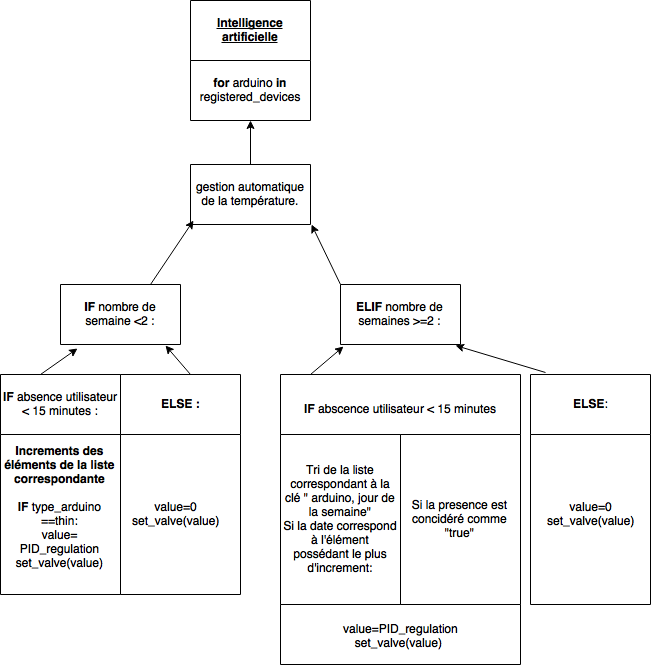
\includegraphics[scale = 0.7]{diagramme_thermo.png}
\caption{\label{thermo} Diagramme de l'algorithme composant l'intelligence artificielle}
\end{figure}
\begin{comment}
Concernant la partie \textbf{smart} du projet, nous avons pensé à plusieurs idées intéressantes qui pourraient améliorer l'expérience de l'utilisateur. En effet ce chapitre met en avant toutes les caractéristiques devenues friand dans le monde de la domotique et avec l'avènement des smartphones, de nombreuses applications en liaison avec notre projet pourraient se développer.\\

\noindent 
Voici en outre une liste non exhaustive des différentes améliorations possibles:

\begin{itemize}
\item un contrôle à distance de l'unité centrale via le WWW
\item une application smartphone notifiant des demandes de préchauffage en fonction de l'heure de la journée et/ou de la 		géolocalisation.
\item un apprentissage du comportement de l'utilisateur en vue d'une anticipation dans les périodes de chauffage.
\item des statistiques des pièces les plus souvent exploitées.
\item utiliser les informations de la météo pour conseiller l'utilisateur sur les futurs planning de chauffage
\item incorporer un module caméra au Raspberry Pi et notifier à l'utilisateur lorsqu'un de ses proches rentre au domicile avec une 	photo de celui-ci
\end{itemize}
\end{comment}

\section{Interface d'utilisateur}
Dans cette section, nous allons nous consacrer aux différentes fonctionnalités et interactions possibles pour le contrôle du thermostat par l'utilisateur. Pour commencer, une page web est à la disposition de l'utilisateur via l'adresse suivante: \url{http://192.168.10.1:8080}. Il est nécessaire de se connecter au réseau WiFi du thermostat central pour accéder à cette page ou que celui-ci est connecté au réseau domestique.
Il pourra s'y connecter via n'importe quel navigateur internet et ainsi donc voir la température de chaque pièce dans laquelle se trouve un thermostat individuel. En effet, cette page met à jour la température régulièrement en se basant sur les dernières mesures enregistrées par l'unité centrale dans la base de données. Grâce à cette même page, l'utilisateur sera en mesure de modifier la température de consigne de son bâtiment en fonction de ses besoins. Une autre option permet également d'arrêter le processus de chauffe en cas de nécessité.\\
\vspace{2cm}
\begin{figure}[H]
\centering
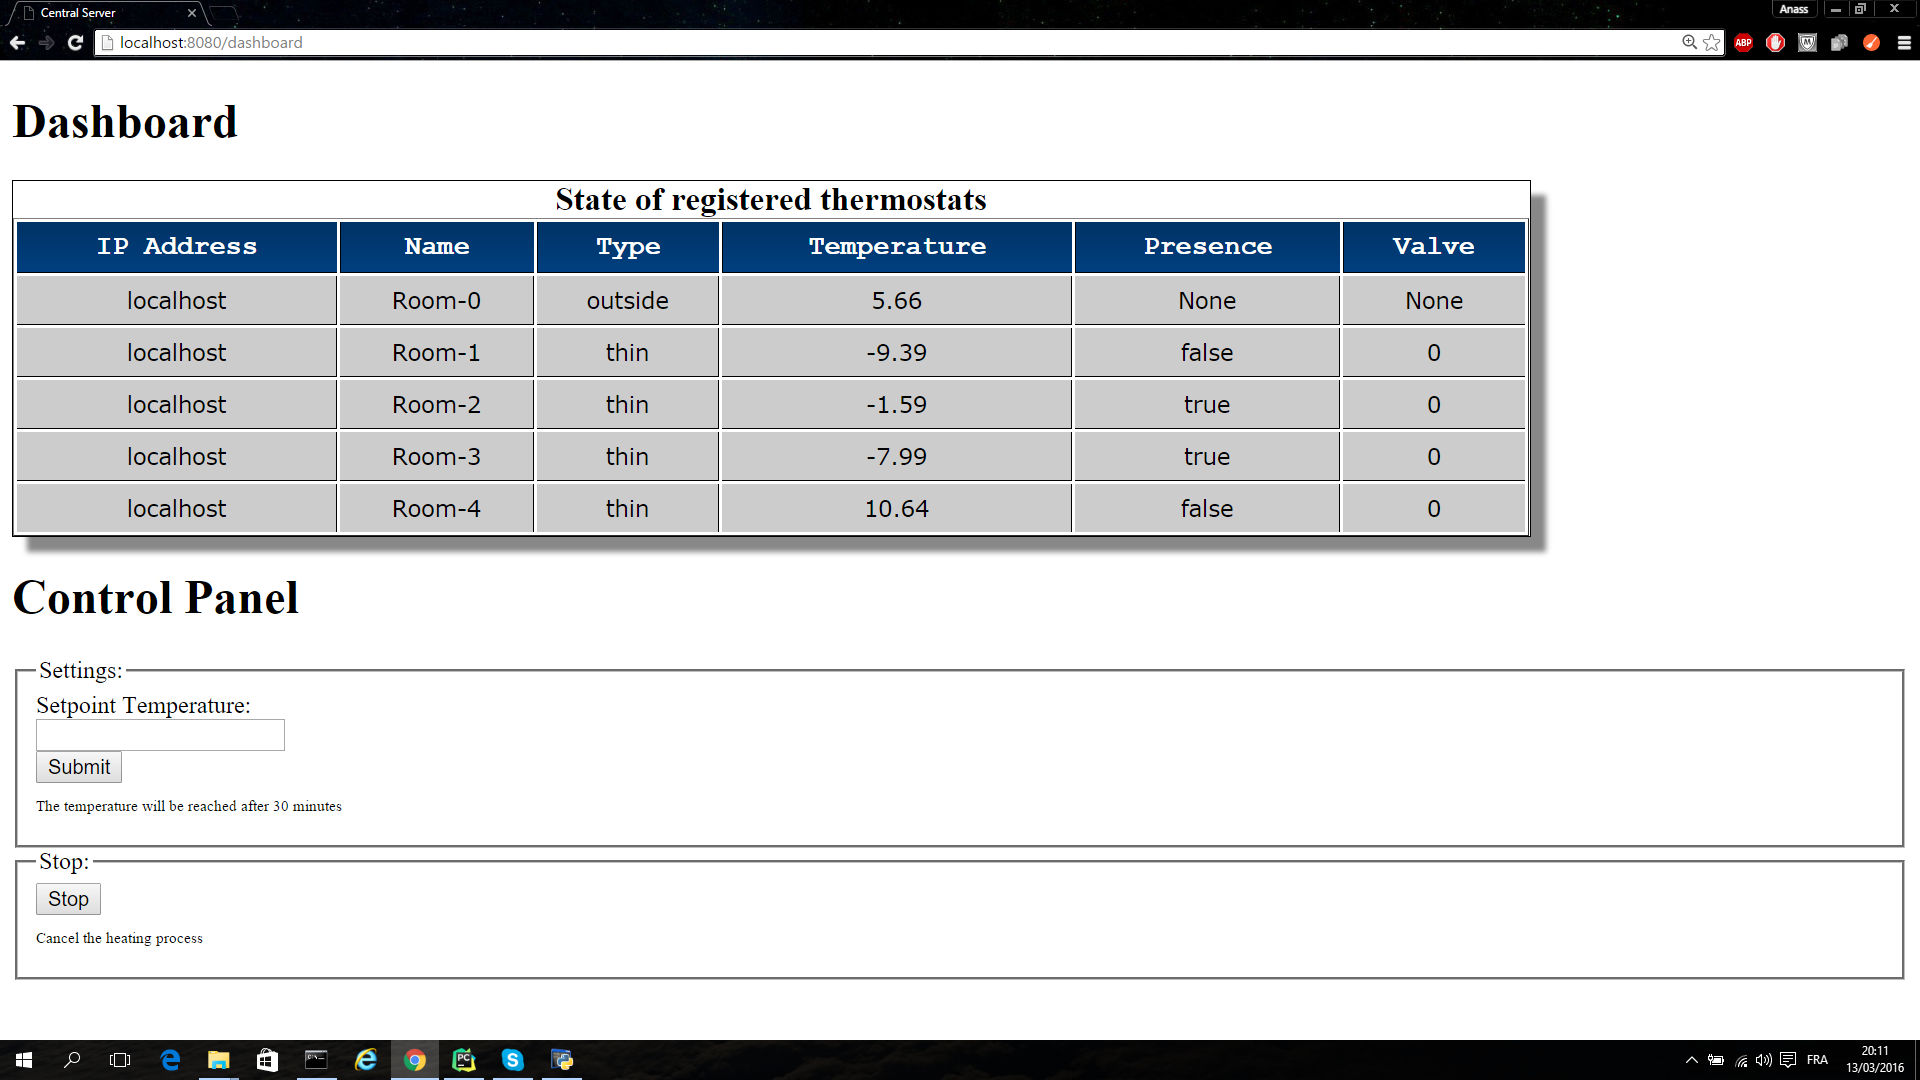
\includegraphics[scale = 0.3]{dashboard.png}
\caption{\label{dashboard} Dashboard}
\end{figure}

\newpage
\noindent
En parallèle, nous avons également mis au point une application Android (figure \ref{android}) simple et intuitive qui permet à l'utilisateur d'avoir un contrôle de son thermostat à partir de son smartphone. Son développent a été possible grâce au logiciel App Inventor 2 \cite{_mit_????} qui est un programme développé par Google et entretenu par le Massachusetts Institute of Technology (MIT). Cette application permet, tout comme la dashboard, de modifier la consigne et afficher la température des différentes pièces de l'immeuble.

\begin{figure}
\centering
\includegraphics[scale = 0.7]{android.png}
\caption{\label{android} Application android}
\end{figure}

\noindent

\chapter{Fonctionnement du groupe}
Cette section du rapport est d\'{e}di\'{e} au fonctionnement du groupe afin d’analyser les points forts et points faibles du groupe responsable de la conception du thermostat et de d\'{e}crire au mieux son organisation.\\

\noindent
La conception d’un thermostat intelligent est un projet n\'{e}cessitant l’apprentissage du travail en \'{e}quipe. Cet apprentissage est important pour tout ing\'{e}nieur ou scientifique qui est amen\'{e} \`{a} collaborer avec plusieurs personnes. Il a donc fallu mettre en place une m\'{e}thode de travail o\`{u} la communication est un \'{e}l\'{e}ment clef notamment pour la r\'{e}partition des t\^{a}ches.\\

\noindent
La communication entre les membres du groupe a \'{e}t\'{e} assur\'{e}e par la mise en place de plusieurs r\'{e}unions organis\'{e}es chaque semaine. Lors de celles-ci deux membres sont désignés pour être soit animateur soit secrétaire. L'animateur a pour r\^ole de donner
la parole et de faire participer tout le monde aux discussions, le secrétaire quant a lui
reprend par écrit les grandes lignes de la réunion. La rédaction de P.V (procès verbal) permettent de rester informé sur les taches à accomplir aux
prochaines réunions ainsi que du lieu et de la date ou se tiendront celles-ci.\\

\noindent
Il a \'{e}t\'{e} pr\'{e}f\'{e}rable de cr\'{e}er un groupe sur le logiciel GIT, un logiciel de gestion de fichier conservant un ensemble de fichiers ainsi que les modifications r\'{e}centes effectu\'{e}es sur ceux-ci. Ce logiciel a permis d’enregistrer chaque proc\`{e}s-verbal r\'{e}dig\'{e} lors des r\'{e}unions et ainsi donc dévoiler une certaine évolution dans l'avancement du projet. Cependant, sur la figure \ref{git}, nous pouvons facilement remarquer que l'utilisation du GIT était assez faible durant le premier quadrimestre, le groupe n'était pas en mesure d'utiliser pleinement les ressources fournies. Néanmoins, nous pouvons remarquer une  augmentation du nombre d'utilisation du GIT. En effet,les échelles des deux graphiques (figure 6.1) sont différentes. Le diagramme "b" du GIT possède une échelle allant au-delà de 10 uploads par jour.\\

\noindent
Les r\'{e}f\'{e}rences des ouvrages utilis\'{e}s ont \'{e}t\'{e} r\'{e}unis gr\^{a}ce au logiciel « Zotero » permettant \`{a} chaque membre de se renseigner sur un sujet \`{a} partir d’un ouvrage fourni par un autre étudiant.\\

\noindent
L'entente des membres du groupe s'est vu améliorée étant donné que ceux-ci appartiennent au groupe 3B de TP et on donc un horaire commun. En raison du  nombre de debuggage à effectuer et au manque de temps du fait de la densité des cours de l'année BA2, plusieurs réunions sans le tuteur ont été planifiées pour se
tenir informe de l'avancement ds travaux des différents membres de l'équipe. Ces réunions avaient pour but d'éclaircir toute incompréhension afin que chaque membre de l'équipe puisse être imprégné de l'état
d'avancement du projet.\\

\noindent
L’\'{e}quipe a connu des moments difficiles \`{a} g\'{e}rer. En effet, suite \`{a} quelques malentendus, certains probl\`{e}mes concernant la conception ou les \'{e}ch\'{e}ances ont \'{e}t\'{e} rencontr\'{e}s. Heureusement,ces probl\'{e}mes ont généralement pu être r\'{e}glés ou contournés grâce à une solution alternative.\\

\noindent
Pour conclure, un plan de travail a \'{e}t\'{e} mis en place lors du premier quadrimestre. Celui-ci a permis au groupe de se projeter sur l'ann\'{e}e afin d'avoir une id\'{e}e globale des diff\'{e}rents volets touchant le projet. Ce plan a \'{e}galement servi \`{a} fixer des \'{e}ch\'{e}ances que l'\'{e}quipe a tent\'{e} de respecter.
Durant le second quadrimestre, nous nous sommes concentrés sur la partie intelligente du projet ainsi que sur la régulation PID du thermostat. On remarque donc que le planning est respecté. Les tâches citées précédemment constituaient la principale préoccupation du groupe sans compter les problèmes de communication entre Raspberry et arduino, le plan de travail n'a donc pas pu être mis à jour.   %modifié car cela à évoluer
 
\begin{center}
\begin{figure}
    \begin{minipage}[t]{8cm}
        \centering
        \subfigure[1er Quadrimestre]{\label{git1}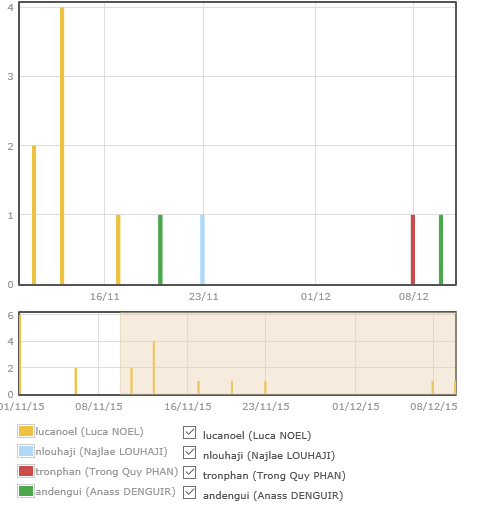
\includegraphics[width=8cm]{post_GIT.png}}
    \end{minipage}\hfill
    \begin{minipage}[t]{8cm}
        \centering
        \subfigure[2ème Quadrimestre]{\label{git2}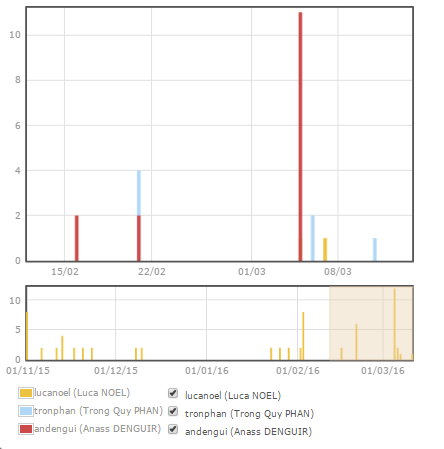
\includegraphics[width=8cm]{Capture2.PNG}}
    \end{minipage}
    \caption{\label{git} Diagrammes du GIT}
\end{figure}
\end{center}

\begin{figure}[H]
\centering
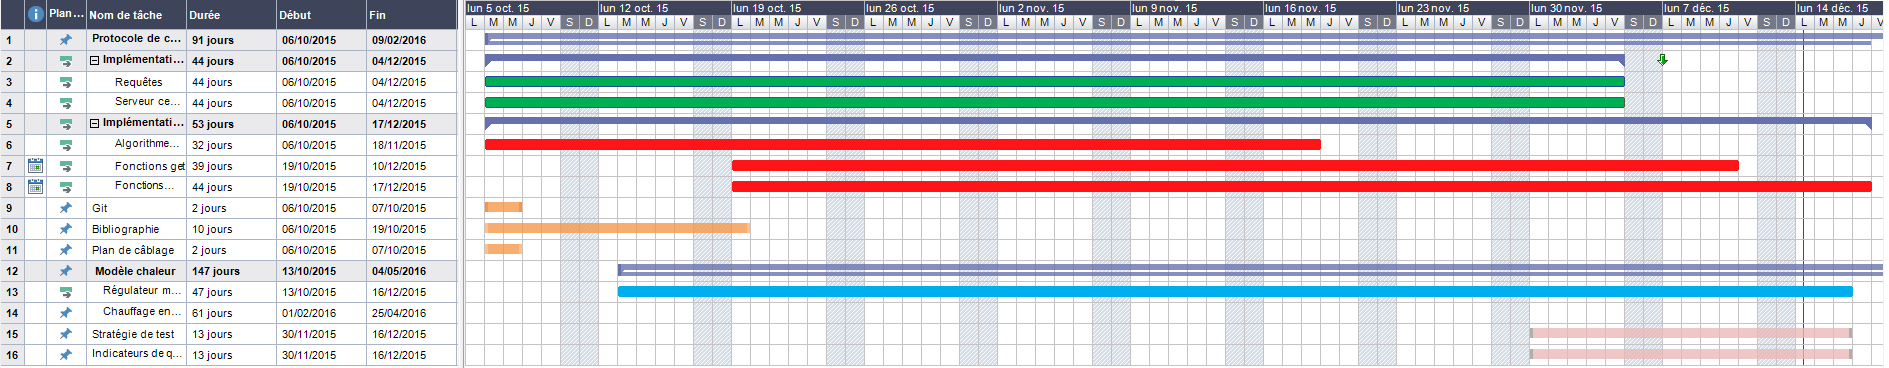
\includegraphics[angle=270, scale = 0.45]{plan_de_travail.PNG}
\caption{\label{plan} Plan de travail}
\end{figure}

\chapter{Conclusion}

Arrivé au terme de ce projet, ce rapport reflète les 6 mois de travail de groupe et son déroulement. Un des plus gros défis dans ce projet a été l'implémentation de l'algorithme pour la régulation de la température en une période de temps très courte. Le choix se portant sur une régulation PID a été très laborieux par le développement d'une phase intermédiaire de calibration afin de trouver des constantes adéquates. En effet, une des grosses difficultés de ce projet résidait dans le fait que les environnements dont la température devait être contrôlée ne possédaient pas des caractéristiques physiques fixes et une loi de comportement thermique connue. Le thermostat intelligent devait donc s'adapter à tout type de pièce. Cette contrainte nous a empêché de développer une simulation informatique de notre environnement dans le but de réaliser nos tests de calibration et de régulation rapidement et non pas sur l'environnement physique de simulation pour lequel un temps de refroidissement était nécessaire entre chaque test.\\
Une autre difficulté et frustration de ce projet a été le débogage du code python lié aux différents problèmes de communication entre les thermostat central et individuels. Ces bugs difficiles à régler étaient assez récurrents et contraignants notamment lorsqu'il était nécessaire de réguler la température durant une journée ou tester notre intelligence artificielle sur une longue période de temps.\\
Ce projet multidisciplinaire touchant à sa fin, nous pouvons tirer une leçon sur les différentes erreurs commises durant l'année en particulier lors du premier quadrimestre. La gestion du temps imposé a probablement été notre plus grand point faible ainsi que notre négligence lors de la présentation de mi-parcours.\\
Malgré tout, cela fut une expérience très enrichissante nous montrant d'autres aspects dans le domaine de l'informatique, l'électronique, la domotique et la gestion de projet. Ce travail nous a également permis de développer notre esprit d'ingénieur, en effet un ingénieur se doit de trouver une solution optimale à son problème et le plus rapidement possible.\\
Enfin ce projet n'étant pas totalement optimisé, des améliorations et innovations sont parfaitement envisageables tant bien au niveau de la communication, de l'intelligence artificielle ou encore de l'interface d'utilisateur.

\addcontentsline{toc}{chapter}{Bibliographie}
\bibliographystyle{plain}
\bibliography{biblio}

\appendix

\chapter{Rapport de recherche bibliographique}

La r\'{e}alisation d'un thermostat intelligent nécessite des renseignements sur l'aspect informatique du projet comprenant, par exemple, les algorithmes de contr\^{o}le ainsi que les constructions de circuits \'{e}lectriques \`{a} produire.
\newline
Une recherche bibliographique semble donc indispensable . Les \'{e}quations de recherche ont permis de trouver les sources que les membres du groupes ont d\'{e}cid\'{e} de s\'{e}lectionner. Ces \'{e}quations ont \'{e}t\'{e} cr\'{e}\'{e} en se basant sur les mots-cl\'{e} provenant du cahier des charges. Les sources s\'{e}lectionn\'{e}s sont accompagn\'{e}s , dans ce document, des motivations de s\'{e}lection. Ce document se conclut par la bibliographie. Celle-ci contient chaque d\'{e}tails de sources choisis.  
\section{Ressources consult\'{e}es}
Bureau d'appui p\'{e}dagogique de l'\'{e}cole polytechnique (BAPP),
Google, Wikip\'{e}dia, catalogue de l'ULB (CIBLE +), Technique de l'ing\'{e}nieur.
\section{Mots-cl\'{e}s}

\subsection{Keywords}
Thermostat, sensor, actuator, Raspberry Pi, Arduino, Wi-Fi module (ESP8266), thermal inertia,  thermistor, power resistor, hypertext transfert protocol, server, python, communication protocol, database,implementation, controller algorithm, on-off.

\subsection{Traduction des mots-cl\'{e}s}
Thermostat, capteur, actionneur, Raspberry Pi, Arduino, module Wi-Fi(ESP8266), inertie
thermique, thermistor, r\'{e}sistance de puissance, hypertext transfert protocol, serveur, python, protocole de communication, base de donn\'{e}es,impl\'{e}mentation, algorithme de contr\^{o}le, on-off.

\vspace{1.5cm}
\begin{center}
\begin{tabular}{|c|c|}
\hline
{\uline{{\Huge Mots-cl\'{e}s.}}}&{\uline{{\Huge Keywords.}}}\\
\hline
{\large Thermostat individuel}&{\large Thin thermostat}\\
\hline
{\large Capteur}&{\large Sensor}\\
\hline
{\large Actionneur}&{\large Actuator}\\
\hline
{\large Raspberry Pi}&{\large Raspberry Pi}\\
\hline
{\large Arduino}&{\large Arduino}\\
\hline
{\large Module Wi-Fi (ESP8266)}&{\large Wi-Fi module (ESP8266)}\\
\hline
{\large Inertie thermique}&{\large Thermal inertia}\\
\hline
{\large Thermistor}&{\large Thermistor}\\
\hline
{\large Resistance de puissance}&{\large Power resistor}\\
\hline
{\large World Wide Web}&{\large World Wide Web}\\
\hline
{\large Thermostat central}&{\large Central thermostat}\\
\hline
{\large Hypertext transfert protocol}&{\large Hypertext transfert protocol}\\
\hline
{\large Serveur}&{\large Server}\\
\hline
{\large Python}&{\large Python}\\
\hline
{\large Protocol de communication}&{\large Communication protocol}\\
\hline
{\large Base de donn\'{e}es}&{\large Database}\\
\hline
{\large Impl\'{e}mentation}&{\large Implementation}\\
\hline
{\large Algorithme de contr\^{o}le}&{\large Controller algorithm}\\
\hline
{\large On-Off}&{\large On-Off}\\ 
\hline
\end{tabular}
\end{center}
\section{Sources s\'{e}lectionn\'{e}es}
\textbf{The Raspberry Pi Foundation. \textit{Help Guides and resources - how to
use raspberry-pi. }} \cite{_raspberry_????}

Lors de la r\'{e}alisatson du thermostat intelligent, la compr\'{e}hension du
fonctionnement du Raspberry Pi sera n\'{e}cessaire.  Ce document nous permettra
de nous renseigner sur la mani\`{e}re efficace d'exploiter l'appareil. La
documentation est fournie par les d\'{e}veloppeurs du Raspberry PI. La
validit\'{e} de la source est donc v\'{e}rifi\'{e}e.
\vspace*{1cm}

\textbf{National instruments. \textit{Types de capteurs de temp\'{e}rature. }} \cite{_types_????}


\textbf{Wikip\'{e}dia,\textit{ Capteur}} \cite{_capteur_2015}

L'utilisation de capteur thermique ou thermistor fera l'objet de plusieurs
recherches. Le groupe devra notamment rechercher le type de capteurs auquel il
fait face, se renseigner sur son fonctionnement ainsi que sur l'exploitation des
donn\'{e}es fournies par le capteur.


La validit\'{e} d'un site tel que Wikip\'{e}dia n'est pas assur\'{e}e.
N\'{e}anmoins, le contenu des documents trouv\'{e}s sur la page web est fort
similaire aux documents fournis par National instruments. On peut donc juger la source de
Wikip\'{e}dia comme valide.

\vspace*{1cm}
\textbf{MCROBERTS Michael. \textit{Beginning Arduino.}} \cite{mcroberts_michael_beginning_2013}


\textbf{FITZGERALD Scott. Mai 2013.  \textit{Arduino project book.}}\cite{_arduino_2013}
\vspace*{1cm}


 Le Raspberry Pi utilis\'{e} durant le projet sera reli\'{e} \`{a} un ou
plusieurs thermostats individuels. Une carte Arduino permettra \`{a} un
thermostat de r\'{e}aliser ses fonctions ainsi que d'envoyer des donn\'{e}es au
Raspberry PI  consed\'{e}r\'{e} ici comme un thermostat central. L'\'{e}tude
de son fonctionnement ainsi que de son langage de programmation seront donc
n\'{e}cessaires durant la r\'{e}alisation d'un thermostat individuel.
On peut considérer la source comme valide. En effet, il s'agit du livre écrit par l'organisme Arduino afin de donnles connaissances de base aux utilisateurs.

\vspace*{1cm}
\textbf{HAELTERMAN Marc. 2014.\textit{ Physique g\'{e}n\'{e}ral~: Syllabus de
laboratoire.}} \cite{haelterman_marc_physique_2014}

La cr\'{e}ation de circuit \'{e}lectrique fera partie de la conception du
thermostat intelligent. Les informations du cours de physique g\'{e}n\'{e}ral
seront donc utiles \`{a} la construction. Le syllabus de laboratoire comprend la
description de deux manipulations de circuit \'{e}lectriques.
Ce syllabus était proposé aux étudiants par le professeur Marc HAELTERMAN durant l'année 2014-2015. On peut considérer le document pertinent.

\vspace*{1cm}

\textbf{{\textit{Requests: HTTP for Humans}}} \cite{_requests:_????}

La librairie "request",inclue dans le programme python, servira à la communication entre les thermostats individuels et le Raspberry Pi. La compr\'{e}hension  du package nous permettra de r\'{e}aliser la distribution de donn\'{e}es entre les deux composantes. Le site est propos\'{e} par le tuteur du groupe ainsi que par le cahier des charges. Il contient des exemples de r\'{e}alisation de programme et des explications permettant un apprentissage rapide et efficace. 
Cette source est proposée par les rédacteurs de l'énoncé du projet. On conclut donc la pertinence du site.

\vspace*{1cm}
\textbf{\textit{HTML5 A vocabulary and associated APIs for HTML and XHTML}} \cite{_html5_????}

Lors des \'{e}changes de donn\'{e}es entre le Raspberry Pi et les thermostats individuels, le Raspberry servira de serveur. Les thermostats individuels enverront donc leurs requ\^{e}tes au serveur. Il est donc nécessaire de pouvoir g\'{e}rer des pages html.
Le site consult\'{e} est propos\'{e} et cr\'{e}er par le World Wide Web Consortium qui est une communauté international. Cela permet de vérifier la validité du document. Il traite le sujet du HTML et permet de s\'{e}lectionner des informations int\'{e}ressantes bien que, dans le cadre de ce projet, la gestion du serveur se fera via python.
 

\vspace*{1cm}
\textbf{\textit{Apprendre \`{a} programmer avec {Python} 3.}}\cite{swimmen_gerard_apprendre_2012}

Le document de G\'{e}rard Swimmen servira de rappel mais renseignera \'{e}galement les membres du groupe sur les modules inclus dans python. Il sera également d'une grande aide en ce qui concerne la conception d'un serveur.
Il s'agit d'un document didactique conseill\'{e} par Thierry Massart, professeur d'informatique \`{a} l'universit\'{e} libre de Bruxelles. 
\vspace*{1cm}

\textbf{\textit{Bottle: Python Web Framework}} \cite{_bottle:_????}

Bottle est un module python qui permet en seulement quelques commandes d'impl\'{e}menter un serveur. Il comporte \'{e}galement quelques m\'{e}thodes utiles telles que GET et POST qui permettent d'int\'{e}ragir avec ce dernier.L'utilisation de ce module ainsi que les sources li\'{e}es \`{a} celui-ci a mentionn\'{e}e dans le cahier des charges. Ce site est proposé par les rédacteurs de l'énoncé du projet.
\vspace*{1cm}

\textbf{\textit{SQlite3 interface for SQLite databases}}\cite{_11.13._????}

SQlite3 est une librairie Python qui sert \`{a} l'impl\'{e}mentation de base de donn\'{e}es.
Ces derni\`{e}res serviront notamment à g\'{e}rer les diverses informations communiqu\'{e}es par les capteurs.
SQlite est simple d'utilisation et d\'{e}j\`{a} install\'{e} par d\'{e}faut sur python, ce qui facilite son utilisation.
La pertinence du document est certifié car l'organisme python est à l'origine de celui-ci.


\vspace*{1cm}
\textbf{\textit{JSON}} \cite{_json_????}

Json est un texte format\'{e} qui sert \`{a} la communication entre le serveur et les diff\'{e}rents thermostats individuels.
Ce langage est particuli\`{e}rement utile car il pr\'{e}sente une structure similaire \`{a} celle des langages de programmation tel que python.
Ce site a \'{e}t\'{e} conseill\'{e} dans le cahier des charges.
\vspace*{1cm}

\textbf{\textit{Automatisme et r\'{e}gulation des \'{e}quipements thermiques}} \cite{bourgeois_automatisme_2015}

\textbf{\textit{M\'{e}thodes d'optimisation pour le r\'{e}glages de contr\^{o}leurs PID}} \cite{de_geest_emmanuel_methodes_????}

Il est souhait\'{e} que, lorsque l'un des thermostat individuel chauffe l'environnement physique, nous n'observions pas une oscillation de la temp\'{e}rature au niveau de la temp\'{e}rature de consigne. Il faut donc cr\'{e}er un algorithme de contr\^{o}le bas\'{e} sur certaines mod\'{e}lisations.
"Automatisme et r\'{e}gulation des \'{e}quipements thermiques" nous renseigne sur le fonctionnent du PID.Il s'agit d'un document provenant du site "techniques ing\'{e}nieur" connu pour ses sources fiables. "M\'{e}thodes d'optimisation pour le r\'{e}glages de contr\^{o}leurs PID" nous donne chaque details concernant le PID. Ce document est un m\'{e}moire d'un ing\'{e}nieur diplom\'{e} de l'universit\'{e} de Li\`{e}ge.
\vspace*{1cm}


\textbf{\textit{NTC Thermistor, radial leaded, standard precision}} \cite{100.pdf_????}

Le calcul de la temp\'{e}rature par le thermostat individuel sera effectu\'{e} gr\^{a}ce \`{a} un thermistor. Le fichier PDF est fourni par Vishay.com, un site sp\'{e}cialis\'{e} dans la vente de mat\'{e}riels \'{e}lectronique. Le document donne des renseignements tel que l'algorithme de conversion de bit en temp\'{e}rature ce qui sera utile \`{a} la conception du thermostat.
\section{Equations de recherches}
\textit{Help Guides and ressources - how to
use raspberry-pi.}:

Raspberry pi AND Tutorial

\vspace*{0.3cm}

\textit{Types de capteurs de temp\'{e}rature}\textit{.~}:

Sensor AND categories

\vspace*{0.3cm}

\textit{ G\'{e}n\'{e}ralit\'{e}s sur les capteurs.~}:


Sensor AND categories

\vspace*{0.3cm}

\textit{Capteur}\textit{~}:

Sensor

\vspace*{0.3cm}


\textit{NTC Thermistor, radial leaded, standard precision:} 

thermostat AND sensor AND Arduino
\vspace*{0.3cm}

\textit{Automatisme et r\'{e}gulation des \'{e}quipements thermiques:}

thermal inertia AND regulation
\vspace*{0.3cm}


\textit{HTML5 A vocabulary and associated APIs for HTML and XHTML:}

HTML AND World Wide Web

\vspace*{0.3cm}

\textit{Requests: HTTP for Humans}:

Python AND Communication protocol

\vspace*{0.3cm}

\textit{Bottle: Python Web Framework}:

Python AND Server AND World Wide Web

\vspace*{0.3cm}

\textit{SQlite3 interface for SQLite databases}:

Python AND Database

\vspace*{0.3cm}

\textit{JSON}:

Python AND Communication protocol

\vspace*{0.3cm}

\textit{Automatisme et r\'{e}gulation des \'{e}quipements thermiques}:

Implementation AND thermostat AND Controller algorithm

\vspace*{0.3cm}

\textit{M\'{e}thodes d'optimisation pour le r\'{e}glages de contr\^{o}leurs PID}:

Implementation AND Controller algorithm AND On-Off

\chapter{Information sur le groupe}

\begin{minipage}{0.4\textwidth}
        \begin{center} \large
        	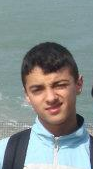
\includegraphics[scale=1.3]{Anass.PNG}\\
            \small DENGUIR Anass\\
			\small 000408788\\
			\small andengui@ulb.ac.be
            \end{center}
            \end{minipage}\hfill
            \begin{minipage}{0.4\textwidth}
            \begin{center} \large
            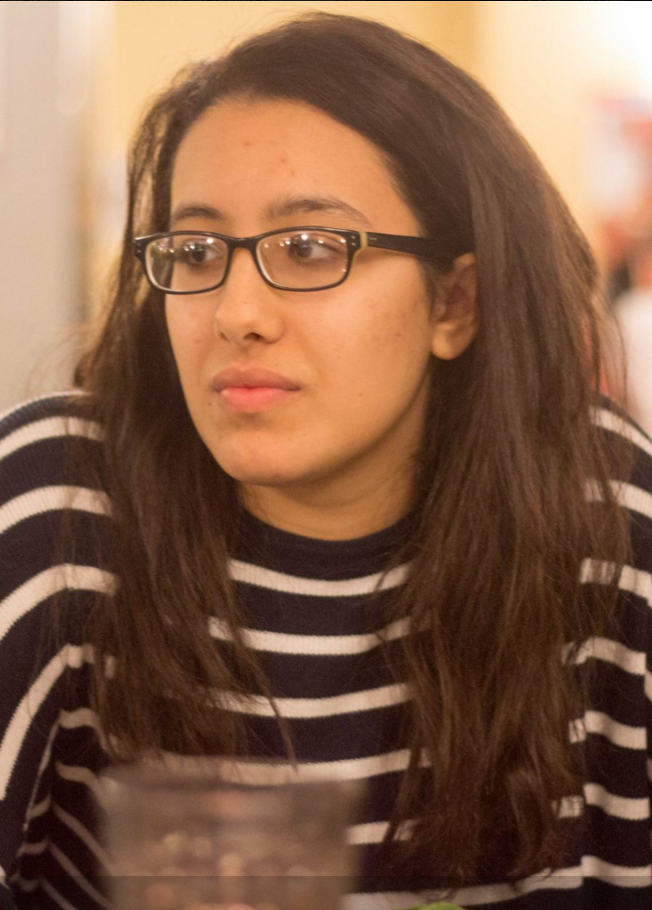
\includegraphics[scale=0.24]{Najlae.PNG}\\
            \small LOUHAJI Najlae\\  
            \small 000408719\\
            \small Najlae.Louhaji@ulb.ac.be
        \end{center}
    \end{minipage}\\[1 cm]

\vspace{1cm}

\begin{minipage}{0.4\textwidth}
        \begin{center} \large
        	
\includegraphics[scale=0.25]{Luca.PNG}\\
            \small NOEL Luca\\
			\small 000407261\\
			\small Luca.Noel@ulb.ac.be
            \end{center}
            \end{minipage}\hfill
            \begin{minipage}{0.4\textwidth}
            \begin{center} \large
            
\includegraphics[scale=0.08]{Quy.jpg}\\
            \small PHAN Trong Quy\\                             
            \small 000413033\\
            \small tronphan@ulb.ac.be
        \end{center}
    \end{minipage}
\end{document}
